\chapter{Applications of Integrals}
%Begin Section 8.1
\section{Area Between Curves}
The ``area under a curve'' was defined in Chapter 5 as the area below some curve
$y=f(x)$ and above the $x$-axis over some interval. That was a special case of
the \textbf{area between curves}\index{area between curves}, where in general
one curve $y=f_1(x)$ is not necessarily always above another curve $y=f_2(x)$
over the entire interval, as in Figure \ref{fig:areacurves} for an interval
$\ival{a}{b}$.

\begin{figure}[h]
\centering
\begin{tikzpicture}[>=latex,every node/.style={font=\small}]
 \path[name path=f1] (1,0.5) parabola bend (6,2.5) (11,0.5);
 \path[name path=f2] (1,2.5) parabola bend (6,0.5) (11,2.5);
 \draw[<->,black!60,line width=1pt,anchor=base] (0,2.6) node[above] {$y$} |- (12,0)
  node[right] {$x$}
  node[black,shift={(0,-0.4)}] at (1,0) {$a$}
  node[black,shift={(0,-0.4)}] at (11,0) {$b$}
  node[black,shift={(0,-0.4)}] at (5.75,0) {$x$}
  node[black,shift={(0.35,-0.4)}] at (6.2,0) {$x+\dx$};
 \draw[black!60] (1,0.1) -- (1,-0.1);
 \draw[black!60] (5.75,0.1) -- (5.75,-0.1);
 \draw[black!60] (6.2,0.1) -- (6.2,-0.1);
 \draw[black!60] (11,0.1) -- (11,-0.1);
 \fill[fill=fillcolor] (1,0.5) parabola bend (6,2.5) (11,0.5)
  -- (11,2.5) parabola bend (6,0.5) (1,2.5) -- cycle;
 \fill[opacity=0.3,fillcolor2] (5.75,0.5) -- (5.75,2.5) -- (6.2,2.5) -- (6.2,0.5) -- cycle;
 \draw[dashed] (1,0.5) -- (1,2.5);
 \draw[dashed] (11,0.5) -- (11,2.5);
 \draw (5.75,0.5) -- (5.75,2.5);
 \draw (6.2,0.5) -- (6.2,2.5);
 \draw[linecolor,line width=1.5pt,name intersections={of=f1 and f2,by={{c,d}}}]
  (1,0.5) parabola bend (6,2.5) (11,0.5);
 \draw[linecolor2,line width=1.5pt] (1,2.5) parabola bend (6,0.5) (11,2.5);
 \node[below left] at (0,0) {$0$};
 \fill (1,0.5) circle (2.5pt);
 \fill (1,2.5) circle (2.5pt);
 \fill (11,0.5) circle (2.5pt);
 \fill (11,2.5) circle (2.5pt);
 \node[left] at (4,0.6) {$y=f_2(x)$};
 \node[left] at (4,2.4) {$y=f_1(x)$};
 \node at (6,1.9) {$\dA$};
 \node[right] at (6.15,1.5) {$h(x)=\abs{f_1(x)-f_2(x)}$};
 \draw[->] (6.45,1.7) -- (6.45,2.4);
 \draw[->] (6.45,1.3) -- (6.45,0.6);
 \draw[->|] (5.45,2.7) -- (5.75,2.7);
 \draw[->|] (6.5,2.7) -- (6.2,2.7);
 \node at (5.975,2.7) {$\dx$};
\end{tikzpicture}
\caption[]{\enskip The area $A$ between two curves $y=f_1(x)$ and $y=f_2(x)$ over $\ival{a}{b}$}
\label{fig:areacurves}
\end{figure}

The area $A$ of the region between the curves in Figure \ref{fig:areacurves}
cannot be negative. Thus, a typical infinitesimal area element $\dA$ of the
region is of the form $h(x)\,\dx$, where the \textbf{height function} $h(x)$ is
the nonnegative difference in the $y$-coordinates of the curves at each $x$ in
$\ival{a}{b}$: $h(x) = \Abs{f_1(x) - f_2(x)}$. Hence:\index{height function}

\statethm{thm:areacurves}{The area $A$ between two curves $y=f_1(x)$ and
$y=f_2(x)$ over an interval $\ival{a}{b}$ is:
\begin{equation}\label{eqn:areacurves}
A ~=~ \int_a^b\;\dA ~=~ \int_a^b ~\Abs{f_1(x) - f_2(x)}~\dx
\end{equation}
The interval $\ival{a}{b}$ can be replaced by any interval---finite or
infinite---over which the integral is defined. Neither curve is required to be
above the $x$-axis.}
\newpage
\begin{exmp}\label{exmp:areacurves1}
\parpic[r]{\begin{tikzpicture}[>=latex,every node/.style={font=\small}]
 \fill[fill=fillcolor] (0,1) -- plot[domain=0:2,samples=100] (\x,{exp(0.3*\x)}) -- (2,0)
   -- (0,0) -- cycle;
 \fill[fill=white] (0,1) -- plot[domain=0:2,samples=100] (\x,{exp(-0.3*\x)}) -- (2,0)
   -- (0,0) -- cycle;
 \draw[dashed] (2,1.822) -- (2,0.549) node[midway,right] {$h(x)$};;
 \draw[->,black!60,line width=1pt] (0,0) -- (0,2) node[above] {$y$};
 \draw[->,black!60,line width=1pt,anchor=base] (-1,0) -- (2.5,0) node[right] {$x$}
  node[black,shift={(0,-0.3)}] at (0,0) {$0$}
  node[black,shift={(0,-0.3)}] at (2,0) {$2$};
 \draw[linecolor,line width=1.5pt,domain=-0.8:2,samples=100] plot (\x,{exp(0.3*\x)});
 \draw[linecolor2,line width=1.5pt,domain=-0.8:2,samples=100] plot (\x,{exp(-0.3*\x)});
 \node[left] at (2,2) {$y=e^x$};
 \node[left] at (2,0.3) {$y=e^{-x}$};
\end{tikzpicture}}
\noindent Find the area between $y=e^{x}$ and $y=e^{-x}$ over
$\ival{0}{2}$.\vspace{1mm}
\par\noindent\emph{Solution:} Since $e^x \ge e^{-x}$ for $x$ in $\ival{0}{2}$,
the height function $h(x)$ for the region between the curves over $\ival{0}{2}$
is $h(x)=\Abs{e^x - e^{-x}}=e^x - e^{-x}$. The area $A$ of the region is thus
\begin{align*}
A ~&=~ \int_0^2 ~(e^x - e^{-x})~\dx\\[4pt]
&=~ e^x + e^{-x}~\Biggr|_0^2 ~=~ e^2 + e^{-2} ~-~ (1 + 1)\\
&=~ 2\,(\cosh\,2 \;-\; 1) ~.
\end{align*}
\end{exmp}
\begin{exmp}\label{exmp:areacurves2}
\parpic[r]{\begin{tikzpicture}[>=latex,every node/.style={font=\small}]
 \fill[fill=fillcolor] (0,0) -- plot[domain=0:1,samples=100] (\x,{\x*\x)}) -- cycle;
 \draw[->,black!60,line width=1pt] (0,-0.5) -- (0,1.5) node[above] {$y$};
 \draw[->,black!60,line width=1pt,anchor=base] (-1,0) -- (2,0) node[right] {$x$}
  node[black,shift={(0.2,-0.3)}] at (0,0) {$0$}
  node[black,shift={(0,-0.3)}] at (1,0) {$1$};
 \draw[linecolor,line width=1.5pt] plot[domain=-0.9:1.2,samples=100] (\x,{\x*\x)});
 \draw[linecolor2,line width=1.5pt] (-0.4,-0.4) -- (1.4,1.4)
  node[black,sloped,pos=0.6,above] {$y=x$};
 \node[right] at (0.7,0.49) {$y=x^2$};
\end{tikzpicture}}
\noindent Find the area of the region bounded by $y=x^2$ and $y=x$.\vspace{1mm}
\par\noindent\emph{Solution:} A ``bounded'' region will always mean a region of
finite area, as opposed to unbounded regions. The curves
$y=x^2$ and $y=x$ intersect at $x=0$ and $x=1$, so the region the curves bound
is the shaded region shown in the figure on the right. Since $x \ge x^2$ for
$0 \le x \le 1$, then the height function for the region is
$h(x)=\abs{x^2-x}=x-x^2$. The region's area $A$ is then
\begin{align*}
A ~&=~ \int_0^1 ~(x - x^2)~\dx\\[4pt]
&=~ \frac{1}{2}\,x - \frac{1}{3}\,x^2~\Biggr|_0^1 ~=~ 
\frac{1}{2} - \frac{1}{3} ~=~ \frac{1}{6} ~.
\end{align*}
\end{exmp}
\begin{exmp}\label{exmp:areacurves3}
\parpic[r]{\begin{tikzpicture}[>=latex,every node/.style={font=\small},scale=1.5]
 \fill[fill=fillcolor] (0,0) -- plot[domain=0:pi/3,samples=100] (\x,{sin(\x r)}) -- (1.047,0.5)
  -- plot[domain=pi/3:0,samples=100] (\x,{cos(\x r)}) -- cycle;
 \draw[dashed] (1.047,0.5) -- (1.047,0.866);
 \draw[linecolor,line width=1.5pt] plot[domain=0:pi/3,samples=100] (\x,{sin(\x r)});
 \draw[linecolor2,line width=1.5pt] plot[domain=0:pi/3,samples=100] (\x,{cos(\x r)});
 \draw[<->,black!60,line width=1pt,anchor=base] (0,1.5) node[above] {$y$} |-
  (2,0) node[right] {$x$}
  node[black,shift={(0.2,-0.4)}] at (0,0) {$0$}
  node[black,shift={(0,-0.4)}] at (0.785,0) {$\tfrac{\pi}{4}$}
  node[black,shift={(0,-0.4)}] at (1.047,0) {$\tfrac{\pi}{3}$};
 \node[above right] at (1.04,0.85) {$y=\sin\,x$};
 \node[below right] at (1.04,0.5) {$y=\cos\,x$};
 \node[left] at (0,1) {$1$};
 \draw[black!60] (0.785,0.05) -- (0.785,-0.05);
 \draw[black!60] (1.047,0.05) -- (1.047,-0.05);
\end{tikzpicture}}
\noindent Find the area of the region bounded by $y=\sin\,x$ and
$y=\cos\,x$ over $\ival{0}{\pi/3}$.\vspace{1mm}
\par\noindent\emph{Solution:} As shown in the figure on the right, the curves
intersect at $x=\tfrac{\pi}{4}$, and $\cos\,x \ge \sin\,x$ for
$0 \le x \le \tfrac{\pi}{4}$, while $\sin\,x \ge \cos\,x$ for $\tfrac{\pi}{4}
\le x \le \tfrac{\pi}{3}$. The area $A$ of the region thus needs to be split
into two integrals:
\begin{align*}
A ~&=~ \int_0^{\pi/3}~\abs{\sin\,x \;-\; \cos\,x}~\dx\\
&=~ \int_0^{\pi/4} ~(\cos\,x \;-\; \sin\,x)~\dx ~+~ \int_{\pi/4}^{\pi/3} ~(\sin\,x \;-\; \cos\,x)~\dx\\
&=~ \left(\sin\,x \;+\; \cos\,x~\Biggr|_0^{\pi/4}\right) ~+~ 
    \left(-\cos\,x \;-\; \sin\,x~\Biggr|_{\pi/4}^{\pi/3}\right)\\[4pt]
&=~ \left(\frac{1}{\sqrt{2}} + \frac{1}{\sqrt{2}}\right) ~-~ (0 - 1) ~+~
    \left(-\frac{1}{2} - \frac{\sqrt{3}}{2}\right) ~-~
    \left(-\frac{1}{\sqrt{2}} - \frac{1}{\sqrt{2}}\right)\\[4pt]
&=~ \frac{4\sqrt{2} - 3 - \sqrt{3}}{2}
\end{align*}
\end{exmp}
\divider
\newpage
\noindent Formula (\ref{eqn:areacurves}) can be extended to find the area
between any number of curves, by splitting the integral over subintervals with
different height functions.
\begin{exmp}\label{exmp:areacurves4}
\noindent Find the area of the region bounded by $y=6-x^2$, $y=x$ and $y=-5x$
above the $x$-axis.
\parpic[r]{\begin{tikzpicture}[>=latex,every node/.style={font=\small},scale=0.5]
 \fill[fill=fillcolor] (-1,5) -- plot[domain=-1:2,samples=100] (\x,{6 -(\x)^2}) -- (0,0) -- cycle;
 \draw[linecolor,line width=1.5pt] plot[domain=-2.45:2.45,samples=100] (\x,{6 -(\x)^2});
 \draw[linecolor2,line width=1.5pt] (-1.2,6) node[black,left] {$y=-5x$} -- (0,0);
 \draw[linecolor2,line width=1.5pt] (0,0) -- (2.5,2.5) node[black,right] {$y=x$};
 \draw[->,black!60,line width=1pt] (0,0) -- (0,6.8) node[above] {$y$};
 \draw[->,black!60,line width=1pt,anchor=base] (-3,0) -- (3.2,0) node[right] {$x$}
  node[black,shift={(0,-0.4)}] at (0,0) {$0$}
  node[black,shift={(0,-0.4)}] at (-1,0) {$-1$}
  node[black,shift={(0,-0.4)}] at (2,0) {$2$};
 \node[right] at (1.2,5) {$y=6-x^2$};
 \draw[black!60] (-1,0.2) -- (-1,-0.2);
 \draw[black!60] (2,0.2) -- (2,-0.2);
\end{tikzpicture}}
\par\noindent\emph{Solution:} As shown in the figure on the right, above the
$x$-axis the curve $y=6-x^2$ intersects the line $y=x$ at $x=2$ and intersects
the line $y=-5x$ at $x=-1$. Since $6-x^2 \ge -5x$ over $\ival{-1}{0}$ and
$6-x^2 \ge x$ over $\ival{0}{2}$, the area $A$ of the shaded region needs to be
split into two integrals:
\begin{align*}
A ~&=~ \int_{-1}^0~\Abs{6 - x^2 - (-5x)}~\dx ~+~ \int_{0}^2~\Abs{6 - x^2 - x}~\dx\\
&=~ \int_{-1}^0~(6 - x^2 + 5x)~\dx ~+~ \int_{0}^2~(6 - x^2 - x)~\dx\\
&=~ \left(6x -\frac{1}{3}x^3 + \frac{5}{2}x^2~\Biggr|_{-1}^{0}\right) ~+~ 
    \left(6x -\frac{1}{3}x^3 - \frac{1}{2}x^2~\Biggr|_{0}^{2}\right)\\[4pt]
&=~ 0 ~-~ \left(-6 + \frac{1}{3} + \frac{5}{2}\right)  ~+~
    \left(12 - \frac{8}{3} - 2\right) ~-~ 0
~=~ \frac{21}{2}
\end{align*}
\end{exmp}
\divider

\noindent For some areas between curves it might be easier to switch the roles
of $x$ and $y$, so that instead of a vertical height function you would
use a horizontal width function.

\begin{exmp}\label{exmp:areacurves5}
\noindent Find the area of the region bounded by $x=y^2-2$ and $y=x$.
\parpic[r]{\begin{tikzpicture}[>=latex,every node/.style={font=\small},scale=0.75]
 \fill[fill=fillcolor] (2,2) -- plot[domain=2:-1,samples=100] ({(\x)^2 - 2},\x) -- cycle;
 \draw[->,black!60,line width=1pt] (0,-1.3) -- (0,2.2) node[above] {$y$};
 \draw[->,black!60,line width=1pt,anchor=base] (-2.5,0) -- (3,0) node[right] {$x$}
  node[black,shift={(0.2,-0.4)}] at (0,0) {$0$}
  node[black,shift={(-0.25,-0.4)}] at (-2,0) {$-2$}
  node[black,shift={(0,-0.4)}] at (-1,0) {$-1$}
  node[black,shift={(0,-0.4)}] at (2,0) {$2$};
 \draw[<->] (-1.75,0.5) -- (0.4,0.5) node[pos=0.55,above,yshift=-0.1cm] {$w(y)$};
 \draw[linecolor,line width=1.5pt] (2,2) -- plot[domain=2.2:-1.2,samples=100] ({(\x)^2 - 2},\x);
 \draw[linecolor2,line width=1.5pt] (-1.2,-1.2) -- (2.3,2.3);
 \draw[black!60] (-1,0.1) -- (-1,-0.1);
 \draw[black!60] (2,0.1) -- (2,-0.1);
 \node[right] at (1.2,1) {$y=x$};
 \node[left] at (-0.55,1.5) {$x=y^2-2$};
\end{tikzpicture}}
\par\noindent\emph{Solution:} As shown in the figure on the right, the parabola
$x=y^2-2$ intersects the line $y=x$ at $x=-1$ and $x=2$. The region has different
height functions $h(x)$ for $-2 \le x \le -1$ and $-1 \le x \le 2$, so that two
integrals would be required for the area $A$. However, notice that the width
function $w(y)$ has one definition over the entire region between the curves
$x=y^2-2$ and $x=y$: $w(y) = \Abs{y - (y^2-2)} = y - (y^2 -2)$. Thus, instead of
integrating the vertical strips $\dA = h(x)\,\dx$ along the
$x$-axis, integrate the horizontal strips $\dA = w(y)\,\dy$ along the $y$-axis,
from $y=-1$ to $y=2$:
\begin{align*}
A ~&=~ \int_{-1}^2~w(y)~\dy ~=~ \int_{-1}^2\Abs{y - (y^2 - 2)}~\dy\\
&=~ \int_{-1}^2 (y - (y^2 - 2))~\dy\\
&=~ \frac{1}{2}y^2 - \frac{1}{3}y^3 + 2y~\Biggr|_{-1}^{2}\\[4pt]
&=~ \left(2 - \frac{8}{3} + 4\right) ~-~ \left(\frac{1}{2} + \frac{1}{3} - 2\right)
~=~ \frac{9}{2}
\end{align*}
\end{exmp}
\divider
\newpage
\piccaption[]{\label{fig:areacurvespolar}}\parpic[r]{
\begin{tikzpicture}[>=latex,every node/.style={font=\small}]
 \fill[fill=fillcolor] (0,0) -- plot[domain=pi/6:pi/3]
  (xy polar cs:angle=\x r,radius={1 + 1.5*cos(\x r)}) -- cycle;
 \fill[fill=white] (0,0) -- plot[domain=pi/6:pi/3]
  (xy polar cs:angle=\x r,radius={1 + cos(\x r)}) -- cycle;
 \draw[dashed] (30:2.6) node[right] {$\theta=\alpha$} -- (0,0)
  -- (60:2.2) node[above right] {$\theta=\beta$};
 \draw[<->,black!60,line width=1pt] (0,2.5) node[above] {$y$} |- (3,0) node[right] {$x$};
 \draw[linecolor2,line width=1.5pt,domain=pi/6:pi/3,samples=500,smooth]
   plot (xy polar cs:angle=\x r, radius={1 + cos(\x r)});
 \draw[linecolor,line width=1.5pt,domain=pi/6:pi/3,samples=500,smooth]
   plot (xy polar cs:angle=\x r, radius={1 + 1.5*cos(\x r)});
 \node[above] at (44:2.05) {$r_1$};
 \node[below] at (47:1.7) {$r_2$};
 \node[below left] at (0,0) {$O$};
\end{tikzpicture}}
The area between curves given by polar equations can be found similarly. For
example, consider curves $r=r_1(\theta)$ and $r=r_2(\theta)$ with
$r_1(\theta) \ge r_2(\theta)$ when $\alpha \le \theta \le \beta$ as in Figure
\ref{fig:areacurvespolar}. The area $A$ of the region between the curves and
those angles is simply the difference between the ``outer'' and ``inner'' areas,
each given by formula (\ref{eqn:polararea}):
\[
A ~=~ \int_{\alpha}^{\beta} \tfrac{1}{2}\,r_1^2 \dtheta ~-~
\int_{\alpha}^{\beta} \tfrac{1}{2}\,r_2^2 \dtheta ~=~
\int_{\alpha}^{\beta} \tfrac{1}{2}\,(r_1^2 - r_2^2)~\dtheta
\]
In general, to include cases where the ``outer'' and ``inner'' curves switch
positions, take the absolute value of the difference:

\statethm{thm:areacurvespolar}{The area $A$ between two polar curves
$r=r_1(\theta)$ and $r=r_2(\theta)$ for $\alpha \le \theta \le \beta$ is:
\begin{equation}\label{eqn:areacurvespolar}
A ~=~ \int_{\alpha}^{\beta} \tfrac{1}{2}\,\Abs{r_1^2 - r_2^2}~\dtheta
\end{equation}}

\begin{exmp}\label{exmp:areacurves6}
\parpic[r]{\begin{tikzpicture}[>=latex,every node/.style={font=\small}]
 \fill[fill=fillcolor] (0,0) -- plot[domain=pi/6:pi/3]
  (xy polar cs:angle=\x r,radius={2 + 2*cos(\x r)}) -- cycle;
 \fill[fill=white] (0,0) -- plot[domain=pi/6:pi/3]
  (xy polar cs:angle=\x r,radius={2 - 2*cos(\x r)}) -- cycle;
 \draw[dashed] (30:0.268) -- (30:3.732) node[sloped,pos=0.6,below] {$\theta=\frac{\pi}{6}$};
 \draw[dashed] (60:1) -- (60:3) node[sloped,pos=0.6,above] {$\theta=\frac{\pi}{3}$};
 \draw[<->,black!60,line width=1pt] (0,2.5) node[above] {$y$} |- (3,0) node[right] {$x$};
 \draw[linecolor2,line width=1.5pt,domain=pi/6:pi/3,samples=500,smooth]
   plot (xy polar cs:angle=\x r, radius={2 - 2*cos(\x r)});
 \draw[linecolor,line width=1.5pt,domain=pi/6:pi/3,samples=500,smooth]
   plot (xy polar cs:angle=\x r, radius={2 + 2*cos(\x r)});
 \node[above right] at (60:3) {$r=1+\cos \theta$};
 \node[below left] at (0,0) {$O$};
 \node[right] at (25:0.4) {$r=1-\cos \theta$};
\end{tikzpicture}}
\noindent Find the area between $r=1+\cos\,\theta$ and
$r=1-\cos\,\theta$ for $\frac{\pi}{6} \le \theta \le \frac{\pi}{3}$.\vspace{1mm}
\par\noindent\emph{Solution:} Let $r_1(\theta)=1+\cos\,\theta$ and
$r_2(\theta)=1-\cos\,\theta$. Since $r_1(\theta) > r_2(\theta)$ for
$\frac{\pi}{6} \le \theta \le \frac{\pi}{3}$, the area $A$ of the
region (shown in the figure on the right) is
\begin{align*}
A ~&=~ \int_{\pi/6}^{\pi/3} \tfrac{1}{2}\,\Abs{r_1^2 - r_2^2}~\dtheta ~=~
\int_{\pi/6}^{\pi/3} \tfrac{1}{2}\,((1+\cos\,\theta)^2 - (1-\cos\,\theta)^2)~\dtheta\\
&=~ \int_{\pi/6}^{\pi/3} 2\,\cos\,\theta~\dtheta ~=~ 2\,\sin\,\theta~\Biggr|_{\pi/6}^{\pi/3}
~=~ 2\,\left(\frac{\sqrt{3}}{2} - \frac{1}{2}\right) ~=~ \sqrt{3} \;-\; 1
\end{align*}
\end{exmp}
\divider
\vspace{2mm}

\piccaption[]{\label{fig:montecarloarea}}\parpic[r]{
\begin{tikzpicture}[>=latex,every node/.style={font=\small}]
 \draw[<->,black!60,line width=1pt] (0,3) node[above] {$y$} |- (4,0) node[right] {$x$};
 \draw (0.5,0.5) rectangle (3.5,2.5);
 \filldraw[fill=fillcolor,draw=linecolor,line width=1.5pt] plot[smooth cycle]
  coordinates {(1.5,0.9) (2,2) (3,1.7) (2.2,1.3) (2.8,1)};
 \fill (0.8,0.8) circle (1.5pt);
 \fill (1.8,1.3) circle (1.5pt);
 \fill (0.9,2.3) circle (1.5pt);
 \fill (2.5,1.3) circle (1.5pt);
 \fill (1.1,1.4) circle (1.5pt);
 \fill (1.4,1.9) circle (1.5pt);
 \fill (2.1,1) circle (1.5pt);
 \fill (1.8,2.2) circle (1.5pt);
 \fill (2.2,1.7) circle (1.5pt);
 \fill (2.6,2.2) circle (1.5pt);
 \fill (3,2) circle (1.5pt);
 \fill (3.1,1.5) circle (1.5pt);
 \fill (3.3,0.7) circle (1.5pt);
 \fill (1.8,0.6) circle (1.5pt);
 \fill (2.4,0.8) circle (1.5pt);
\end{tikzpicture}}
\textbf{Monte Carlo integration}\index{Monte Carlo integration} is a technique
for approximating the area of a region by taking a large number of random
points in a rectangle that encloses the region (see Figure
\ref{fig:montecarloarea}). The idea is simple:
\[
\frac{\text{\# of points in the region}}{\text{\# of points in the rectangle}}
~\approx~ \frac{\text{area of the region}}{\text{area of the rectangle}}
\]
For example, if $20\%$ of the random points in the rectangle fall inside the
region, then---by randomness---you would expect the area of the region to be
about $20\%$ of the area of the rectangle. The more random points you take, the
better the approximation. Since the area of the rectangle is known, as
well as the number of random points inside the region and the rectangle, the
area of the region is easy to approximate.\index{integration!Monte Carlo}
\newpage
\begin{exmp}\label{exmp:montecarloarea}
\parpic[r]{\begin{tikzpicture}[>=latex,every node/.style={font=\small}]
 \fill[fillcolor] (0,3) -- plot[domain=0:1.0185] (\x,{sqrt(9 - \x*\x)}) --
  plot[domain=1.0185:0.7347] (\x,{exp(\x*\x)}) -- plot[domain=0.7347:0]
  (\x,{2*cos(\x*\x r)}) -- cycle;
 \draw[draw=linecolor,line width=1.5pt] (0:3) arc (0:90:3);
 \draw[draw=linecolor2,line width=1.5pt] (0,2) -- plot[domain=0:1.253,samples=100]
  (\x,{2*cos(\x*\x r)});
 \draw[draw=linecolor3,line width=1.5pt] (0,2) -- plot[domain=0:1.1,samples=100]
  (\x,{exp(\x*\x)}) node[black,above] {$y=e^{x^2}$};
 \draw[<->,black!60,line width=1pt,anchor=base] (0,3.5) node[above] {$y$}
  node[black,left] at (0,1) {$1$}
  node[black,left] at (0,2) {$2$}
  node[black,left] at (0,3) {$3$}
  |- (4,0) node[right] {$x$}
  node[black,shift={(0,-0.3)}] at (0,0) {$0$}
  node[black,shift={(0,-0.3)}] at (1,0) {$1$}
  node[black,shift={(0,-0.3)}] at (2,0) {$2$}
  node[black,shift={(0,-0.3)}] at (3,0) {$3$};
 \draw[line width=1.5pt] (0,0) rectangle (2,3);
 \node[right] at (35:3.1) {$x^2+y^2=9$};
 \node[right] at (0.23,0.7) {$y=2\cos x^2$};
\end{tikzpicture}}
\noindent Use Monte Carlo integration to approximate the area of the region
in the first quadrant above the curves $y=e^{x^2}$ and $y=2\,\cos\,x^2$, and
inside the circle $x^2+y^2=9$.\vspace{1mm}
\par\noindent\emph{Solution:} The region is the shaded area shown in the figure
on the right, enclosed in a rectangle of width $2$ and height $3$. The area of
the rectangle is $6$, and a point $(x,y)$ in the rectangle is inside the region
if only if the following conditions are met:
\[
y ~>~ e^{x^2} \quad\text{and}\quad y ~>~ 2\,\cos\,x^2 \quad\text{and}\quad
x^2 + y^2 ~<~ 9
\]
Notice that these conditions are all in the form of inequalities. The Monte
Carlo integration is then simple to perform in Octave, using 10 million random
points:

\begin{Verbatim}[frame=single, framesep=2mm,
listparameters=\setlength{\topsep}{3pt}\setlength{\partopsep}{1pt}]
octave> N = 1e7;
octave> x = 2*rand(1,N);
octave> y = 3*rand(1,N);
octave> 6*(sum(y > exp(x.^2) & y > 2*cos(x.^2) & x.^2 + y.^2 < 9))/N
ans = 0.94612
\end{Verbatim}
The actual value---accurate to 5 decimal places---is 0.94606.

The \texttt{rand(1,N)} command returns an array of \texttt{N} random numbers
between $0$ and $1$. So the statement \texttt{x = 2*rand(1,N)} stores \texttt{N}
random numbers between $0$ and $2$ in an array for the $x$-coordinates, and the
statement \texttt{y = 3*rand(1,N)} stores \texttt{N} random numbers between $0$
and $3$ in an array for the $y$-coordinates. The statement
\texttt{y > exp(x.\symbol{94}2)} returns a value of $1$ if the condition
$y > e^{x^2}$ is met, $0$ otherwise. Similarly for the statements
\texttt{y > 2*cos(x.\symbol{94}2)} and
\texttt{x.\symbol{94}2 + y.\symbol{94}2 < 9}. Joining those three statements
with \texttt{\&} symbols returns a value of $1$ if all three conditions are met,
$0$ otherwise. The \texttt{sum} command thus counts how many
of the \texttt{N} points are inside the region. Dividing that count by
\texttt{N} gives the ratio of points inside the region, then multiplying
by $6$ (the area of the rectangle) gives the approximate area of the region.

Note that the size of the rectangle can affect the approximation---generally
the larger the rectangle the more points must be used. Note also in this example
that finding the area by using definite integrals would require numerical
integration methods, since $f(x)=e^{x^2}$ and $f(x)=2\,\cos\,x^2$ cannot be
integrated in a closed form. In fact, even finding the points of intersection of
the three curves---in order to split the integrals---would require a numerical
root-finding method (e.g. Newton's method).
\end{exmp}\vspace{-2mm}
\divider
\vspace{2mm}
\startexercises\label{sec8dot1}
{\small
\probs{A}
\par\noindent For Exercises 1-6, find the area of the region bounded by the
 given curves.
\begin{enumerate}[\bfseries 1.]
\begin{multicols}{3}
 \item $y = x^2$ and $y = 2x + 3$
 \item $x = -y^2 + 2y$ and $x = 0$
 \item $y = x^2 - 1$ and $y = x^3 - 1$
\end{multicols}
\begin{multicols}{3}
 \item $y = x^4$ and $y = x$
 \item $x = y^2$ and $x = y + 2$
 \item $y = 4 - 4x^2$ and $y = 1 - x^2$
\end{multicols}
 \item Find the area between $y = 4x - x^2$ and $y = x$ over $\ival{0}{4}$.
 \item Find the area between $y=\cosh\,x$ and $y=\sinh\,x$ over
  $\lival{0}{\infty}$.
 \item Find the area of the region defined by the inequalities
  $0 \le x \le y - x \le 1 - y \le 1$.
 \item Find the area between $r=1+\cos\,\theta$ and $r=2+2\cos\,\theta$.
 \item Find the area between $r=1+\cos\,\theta$ and $r=2+\cos\,\theta$.
\suspend{enumerate}
\probs{B}
\resume{enumerate}[{[\bfseries 1.]}]
\parpic[r]{\begin{tikzpicture}[>=latex,every node/.style={font=\small}]
 \fill[fillcolor] (1,0) -- plot[domain=1:1.581] (\x,{sqrt(\x*\x - 1)}) --
  plot[domain=1.581:2] (\x,{sqrt(4 -\x*\x)}) -- cycle;
 \draw[name path=cir,linecolor,line width=1.5pt] (0:2) arc (0:90:2);
 \draw[name path=hyp,linecolor2,line width=1.5pt] (1,0) -- plot[domain=1:2.5]
  (\x,{sqrt(\x*\x - 1)}) node[black,above] {$x^2-y^2=1$};
 \fill[name intersections={of=cir and hyp,by={P}}] (P) circle (2.5pt);
 \draw[<->,black!60,line width=1pt,anchor=base] (0,2.5) node[above] {$y$}
  node[black,left] at (0,2) {$2$}
  |- (3,0) node[right] {$x$}
  node[black,shift={(0,-0.3)}] at (1,0) {$1$}
  node[black,shift={(0,-0.3)}] at (2,0) {$2$};
 \node[right] at (20:2) {$x^2+y^2=4$};
 \node[below left] at (0,0) {$O$};
 \node[right] at (P) {$~P$};
\end{tikzpicture}}
 \item Find the area of the region in the first quadrant between the unit
  hyperbola $x^2-y^2=1$ and the circle $x^2+y^2=4$ (i.e. the shaded region shown
  in the figure on the right) in two ways:
  \begin{enumerate}[\bfseries (a)]
   \item Integration using formula (\ref{eqn:areacurves}).
   \item Draw a line segment from the origin $O$ to the point of
intersection\\$P$ on the hyperbola, then use the areas of the resulting
circular\\sector and hyperbolic sector, without resorting to integration.\\Does
your answer agree with part (a)? Explain.
  \end{enumerate}
\suspend{enumerate}
\resume{enumerate}[{[\bfseries 1.]}]
 \item\label{exer:fourcircles} Find the area common to the four circles of
  radius 5 shown in Figure \ref{fig:fourcircles}. \emph{(Hint: Use symmetry.)}

\begin{figure}[ht]
\begin{minipage}[b]{5cm}
\begin{center}
\begin{tikzpicture}[>=latex,every node/.style={font=\small}]
 \fill[fillcolor] (0,0) rectangle (1,1);
 \fill[white,even odd rule] (-1,-1) rectangle (2,2) (0,0) circle (1);
 \fill[white,even odd rule] (-1,-1) rectangle (2,2) (0,1) circle (1);
 \fill[white,even odd rule] (-1,-1) rectangle (2,2) (1,0) circle (1);
 \fill[white,even odd rule] (-1,-1) rectangle (2,2) (1,1) circle (1);
 \draw (0,0) circle (1);
 \draw (0,1) circle (1);
 \draw (1,0) circle (1);
 \draw (1,1) circle (1);
 \draw (0,0) -- (0,1) node[left,midway] {$5$} -- (1,1) node[above,midway] {$5$} --
  (1,0) node[right,midway] {$5$} -- (0,0) node[below,midway] {$5$};
\end{tikzpicture}
\vspace{-4mm}
\end{center}
\caption[]{\enskip Exercise \ref{exer:fourcircles}}
\label{fig:fourcircles}
\end{minipage}
\begin{minipage}[b]{10cm}
 \centering
 \subfloat[][\enskip Area $A$]{
 \begin{tikzpicture}[>=latex,every node/.style={font=\small}]
  \fill[fillcolor] (-1,0.5) parabola bend (0,0) (2,2) -- cycle;
  \draw[linecolor2,line width=1.5pt] (-2,0) -- (3,2.5)
   node[black,sloped,midway,above] {$y = mx + b$};
  \draw[linecolor,line width=1.5pt] (-1.5,1.125) parabola bend (0,0) (2.3,2.645);
  \node[right] at (1.1,0.5) {$y = ax^2$};
  \node at (0.1,0.6) {$A$};
 \end{tikzpicture}}
 \quad
 \subfloat[][\enskip Area $T$]{
 \begin{tikzpicture}[>=latex,every node/.style={font=\small}]
  \fill[fillcolor] (-1,0.5) -- (0.5,0.125) -- (2,2) -- cycle;
  \draw (-1,0.5) -- (0.5,0.125) -- (2,2);
  \draw[linecolor,line width=1.5pt] (-1,0.5) parabola bend (0,0) (2,2);
  \draw[linecolor2,line width=1.5pt] (-1,0.5) -- (2,2);
  \node[left] at (-1,0.5) {$B$};
  \node[right] at (2,2) {$C$};
  \node[below] at (0.5,0.125) {$D$};
  \node at (0.3,0.7) {$T$};
  \node[above left] at (0.3,1.1) {$y = mx + b$};
  \node[right] at (1,0.5) {$y = ax^2$};
 \end{tikzpicture}}
 \caption[]{\enskip Exercise \ref{exer:parabolatriangle}}
 \label{fig:parabolatriangle}
\end{minipage}
\end{figure}

 \item\label{exer:parabolatriangle} Let $A$ be the area of the region bounded by
  the parabola $y = ax^2$ and the line $y = mx + b$, where $a$, $m$, and $b$ are
  positive constants (see Figure \ref{fig:parabolatriangle}(a)). Let $T$ be the
  area of the triangle $\triangle\,BCD$, where $B$ and $C$ are where the line
  intersects the parabola, and the point $D$ on the parabola has the same
  $x$-coordinate as the midpoint of the line segment $\overline{BC}$ (see Figure
  \ref{fig:parabolatriangle}(b)). Show that $A = \frac{4}{3}T$.
 \item In Example \ref{exmp:montecarloarea} the region was enclosed in the
  rectangle $R = \lbrace\; (x,y):\; 0 \le x \le 2~,~0 \le y \le 3 \;\rbrace$.
  Use Monte Carlo integration to approximate the area of the region again, using
  a different enclosing rectangle $R$:
  \begin{enumerate}[\bfseries (a)]
   \item $R = \lbrace\; (x,y):\; 0 \le x \le 2~,~1 \le y \le 3 \;\rbrace$
   \item $R = \lbrace\; (x,y):\; 0 \le x \le 3~,~0 \le y \le 3 \;\rbrace$
  \end{enumerate}
  Are the results significantly different than before?
 \item Approximate the area of the region bounded by $y = x^2$ and $y = \cos\,x$
  in two different ways:
  \begin{enumerate}[\bfseries (a)]
   \item Use Monte Carlo integration with 10 million points.
   \item Use a numerical root-finding method to find the points of intersection
    of the curves, then use those points in a numerical integration method to
    find the area.
  \end{enumerate}
\suspend{enumerate}
\probs{C}
\resume{enumerate}[{[\bfseries 1.]}]
 \item A dog is chained to a fixed point at the circular base of a cylindrical
  silo. The silo's radius is $50$ ft and the chain can wrap exactly halfway
  around the silo. How much total area can the dog roam, not counting the area
  inside the silo?
\end{enumerate}
}
\newpage
%Begin Section 8.2
\section{Average Value of a Function}
\piccaption[]{\label{fig:orbit}}\parpic[r]{\begin{tikzpicture}[every node/.style={font=\small}]
 \draw [line width=1.5pt,linecolor] (0,0) ellipse (2.04 and 1.04);
 \fill (1.04,0.896) circle (2.5pt);
 \node[above right] at (1.04,0.896) {planet};
 \draw[dashed] (-0.7,0) -- (1.04,0.896) node[midway,below right] {$d$};
 \node at (-0.7,0) {\ding{88}};
 \node[below] at (-0.7,0) {Sun};
\end{tikzpicture}}

According to Kepler's laws of planetary motion, a planet revolving around the
Sun follows an elliptical orbit, with the Sun at one focus of the ellipse,
as in Figure \ref{fig:orbit}. The distance $d$ between the planet and the Sun
varies over the ellipse, reaching a minimum distance and a maximum distance (by
the Extreme Value Theorem). How would you find the \emph{average} distance
between the planet and the Sun over one complete orbit?\index{average
value}\index{function!average value} The idea is to generalize the usual notion
of an average of numbers.

Recall that for $n$ numbers $x_1$, $x_2$, $\ldots$ , $x_n$ the \emph{average},
denoted by $\bar{x}$, is simply the sum of the numbers divided by how many
numbers there are, namely
\[
\bar{x} ~=~ \frac{x_1 ~+~ x_2 ~+~ \cdots ~+~ x_n}{n} ~.
\]
In statistics $\bar{x}$ is called the \emph{mean} of $x_1$, $x_2$, $\ldots$ ,
$x_n$. This definition makes sense for a finite set of numbers, but in the case
of a planet revolving around the Sun, there are an uncountably infinite number
of distances between the planet and the Sun, making the above definition
impossible to use. A way of taking a sum over an infinite continuum of values is
needed instead. Such a method has already been encountered: the definite
integral, which is merely a sum of a continuum of infinitesimal quantities.

\piccaption[]{\label{fig:favg}\quad $\Delta x_i = x_i-x_{i-1} = (b-a)/n$}\parpic[r]{\begin{tikzpicture}[>=latex,every node/.style={font=\small}]
 \draw[dashed] (1,0) -- (1,1) node[above left,pos=1.0] {$f(x_0)$};
 \draw[dashed] (1.5,0) -- (1.5,1.875) node[above left,pos=1.0] {$f(x_1)$};
 \draw[dashed] (2,0) -- (2,2.5) node[above left,pos=1.0] {$f(x_2)$};
 \draw[dashed] (3.5,0) -- (3.5,2.875) node[above right,pos=1.0] {$f(x_{n-1})$};
 \draw[dashed] (4,0) -- (4,2.5) node[right,pos=1.0] {$f(x_n)$};
 \draw[<->,black!60,line width=1pt,anchor=base] (-0.5,3) node[above] {$y$} |- (5.5,0) node[right] {$x$}
  node[black,shift={(0,-0.4)}] at (0.5,0) {$a=$}
  node[black,shift={(0,-0.4)}] at (1,0) {$x_0$}
  node[black,shift={(0,-0.4)}] at (1.5,0) {$x_1$}
  node[black,shift={(0,-0.4)}] at (2,0) {$x_2$}
  node[black,shift={(0,-0.4)}] at (2.75,0) {$\ldots$}
  node[black,shift={(0,-0.4)}] at (3.5,0) {$x_{n-1}$}
  node[black,shift={(0,-0.4)}] at (4.1,0) {$x_n$}
  node[black,shift={(0,-0.4)}] at (4.6,0) {$=b$};
 \node at (2.75,1) {$\ldots$};
 \begin{scope}[color=linecolor,line width=1.5pt]
  \pgfplothandlerlineto
  \pgfplotfunction{\x}{1,1.01,...,4}{\pgfpointxy{\x}{-0.5*(\x-3)^2+3)}}
  \pgfusepath{stroke}
 \end{scope}
 \fill (1,1) circle (2.5pt);
 \fill (1.5,1.875) circle (2.5pt);
 \fill (2,2.5) circle (2.5pt);
 \fill (3.5,2.875) circle (2.5pt);
 \fill (4,2.5) circle (2.5pt);
 \end{tikzpicture}}
\picskip{11}
To motivate the definition of the average value of a function $f$ over a closed
interval $\ival{a}{b}$, denoted by $\avg{f}$, consider a partition
\[
P ~=~ \lbrace a = x_0 < x_1 < x_2 < \cdots < x_{n-1} < x_n = b \rbrace
\]
that divides $\ival{a}{b}$ into $n$ subintervals
$\ival{x_{i-1}}{x_i}$ of equal length $\Delta x_i = x_i-x_{i-1} = (b-a)/n$,
as in Figure \ref{fig:favg}. The $n$ function values $f(x_1)$, $f(x_2)$,
$\ldots$ , $f(x_n)$ constitute only a finite subset of all the function
values $f(x)$ over $\ival{a}{b}$, so their average would be an
approximation of the true function average $\avg{f}$, namely:\index{$\avg{f}$}
\[
\avg{f} ~\approx~ \frac{f(x_1) ~+~ f(x_2) ~+~ \cdots ~+~ f(x_n)}{n} ~=~
 \sum_{i=1}^n \frac{f(x_i)}{n}
\]
By properties of summations, divide the entire sum by the constant $b-a$ 
and multiply each term in the sum by $b-a$ to get:
\newpage
\[
\avg{f} ~\approx~ \frac{1}{b-a}\,\sum_{i=1}^n f(x_i)\,\cdot\,\frac{b-a}{n} ~=~
\frac{1}{b-a}\,\sum_{i=1}^n f(x_i)\,\Delta x_i
\]
Note that the last summation on the right is just a Riemann sum for the
definite integral $\int_a^b f(x)\,\dx$, with the points $x_i^*$ chosen to be the
right endpoints of the intervals $\ival{x_{i-1}}{x_i}$ for $i=1$ to $n$. Thus,
taking the limit of that sum as $n \to \infty$ (which means including more and
more function values in the average) yields the following definition:

\statedefn{defn:avgvalue}{The \textbf{average value} $\avg{f}$ of a function $f$
over a closed interval $\ival{a}{b}$ is:\footnotemark
\begin{equation}\label{eqn:avgvalue}
\avg{f} ~=~ \frac{1}{b-a}\,\int_a^b\,f(x)~\dx
\end{equation}
}\footnotetext{In some statistics or mathematics texts you might see the notation
$\bar{f}$ for the average value.}

\begin{exmp}\label{exmp:avg1}
\noindent Find the average value of $f(x)=x^2$ over $\ival{0}{1}$.\vspace{1mm}
\par\noindent\emph{Solution:} By definition, with $a=0$ and $b=1$,
\[
\avg{f} ~=~ \frac{1}{1-0}\,\int_0^1\,f(x)~\dx ~=~ \int_0^1\,x^2~\dx ~=~
\frac{x^3}{3}~\Biggr|_0^1 ~=~ \frac{1^3}{3} ~-~ \frac{0^3}{3} ~=~ \frac{1}{3}
\]
Note that this says that if you took all the numbers between 0 and 1 and
squared them, then the average of those squares would be 1/3.
\end{exmp}
\begin{exmp}\label{exmp:avg2}
\noindent Find the average value of $f(x)=x^2$ over $\ival{-1}{1}$.\vspace{1mm}
\par\noindent\emph{Solution:} By definition, with $a=-1$ and $b=1$,
\[
\avg{f} ~=~ \frac{1}{1-(-1)}\,\int_{-1}^1\,f(x)~\dx ~=~ \frac{1}{2}\,\int_{-1}^1\,x^2~\dx ~=~
\frac{x^3}{6}~\Biggr|_{-1}^1 ~=~ \frac{1^3}{6} ~-~ \frac{(-1)^3}{6} ~=~ \frac{1}{3}
\]
Note that this is the same as the average over $\ival{0}{1}$, as shown in the
previous example. This should make sense, since the function $f(x)=x^2$ is
symmetric about the $y$-axis, so the values of $f(x)$ from $\ival{-1}{0}$ are
the same as those from $\ival{0}{1}$. The values from $\ival{-1}{1}$ just
duplicate the values from $\ival{0}{1}$ and hence do not change the average.
\end{exmp}
\begin{exmp}\label{exmp:avg3}
\noindent Find the average value of $f(x)=\sin\,x$ over $\ival{0}{\pi}$.\vspace{1mm}
\par\noindent\emph{Solution:} By definition, with $a=0$ and $b=\pi$,
\[
\avg{f} ~=~ \frac{1}{\pi-0}\,\int_0^{\pi}\,f(x)~\dx ~=~ \frac{1}{\pi}\int_0^{\pi}\,\sin\,x~\dx ~=~
-\frac{1}{\pi}\,\cos\,x~\Biggr|_0^{\pi} ~=~ -\frac{1}{\pi}\,(\cos\,\pi ~-~ \cos\,0) ~=~
-\frac{1}{\pi}\,(-1 - 1) ~=~ \frac{2}{\pi}
\]
\end{exmp}
\divider
\newpage
\begin{exmp}\label{exmp:avg4}
\piccaption[]{\label{fig:avgellipse}\quad $\frac{x^2}{25} + \frac{y^2}{9} = 1$}\parpic[r]{\begin{tikzpicture}[every node/.style={font=\small}]
 \draw[black!60,solid,line width=0.6pt,-latex] (-2.5,0) -- (2.5,0) node[right]
  {$x$};
 \draw[black!60,solid,line width=0.6pt,-latex] (0,-1.5) -- (0,1.6) node[above]
  {$y$};
 \node[below left] at (0,0) {$0$};
 \draw[black!60,line width=0.3pt,shift={(2.09,0)}] (0pt,3pt) -- (0pt,-3pt);
 \draw[black!60,line width=0.3pt,shift={(-2.09,0)}] (0pt,3pt) -- (0pt,-3pt);
 \node [below right] at (2.02,-0.1) {$5$};
 \node [below left] at (-2.02,-0.1) {$-5$};
 \draw[black!60,line width=0.3pt,shift={(0,1.09)}] (-3pt,0pt) -- (3pt,0pt);
 \draw[black!60,line width=0.3pt,shift={(0,-1.09)}] (-3pt,0pt) -- (3pt,0pt);
 \node [above left] at (-0.1,1.02) {$3$};
 \node [below left] at (-0.1,-1.02) {$-3$};
 \draw [line width=1.5pt,linecolor] (0,0) ellipse (2.04 and 1.04);
 \fill (-1.04,0.896) circle (2pt);
 \node [above left] at (-1,0.866) {$(x,y)$};
 \fill (1.3,0) circle (2pt);
 \node [below] at (1.3,0) {$(4,0)$};
 \draw[dashed] (-1.04,0.896) -- (1.3,0) node[above,pos=0.6] {$d$};
\end{tikzpicture}}
\par\noindent Find the average distance from the ellipse
$\frac{x^2}{25} + \frac{y^2}{9} = 1$ to the point $(4,0)$.\vspace{1mm}
\par\noindent\emph{Solution:} Let $d$ represent the distance from any point
$(x,y)$ on the ellipse to the point $(4,0)$, as in Figure \ref{fig:avgellipse}.
If $(x,y)$ is on the ellipse $\frac{x^2}{25} + \frac{y^2}{9} = 1$ then
$y^2 = 9(1 - \frac{x^2}{25}) = \frac{9}{25}(25-x^2)$. So by the distance 
formula, $d$ is given by
\picskip{0}

\vspace{-23mm}
\begin{align*}
d^2 ~&=~ (x-4)^2 ~+~ (y-0)^2 ~=~ (x-4)^2 ~+~ y^2\\
&=~ (x-4)^2 ~+~ \frac{9}{25}(25-x^2)\\[6pt]
&=~ \frac{25(x-4)^2 ~+~ 9(25-x)^2}{25}
~=~ \frac{25x^2 ~-~ 200x ~+~ 400 ~+~ 225 ~-~ 9x^2}{25}\\[6pt]
&=~ \frac{16x^2 ~-~ 200x ~+~ 625}{25}\\[6pt]
d^2 ~&=~ \frac{(4x - 25)^2}{25} \quad\text{, and so taking square roots gives}\\[6pt]
d ~&=~ \pm\,\frac{4x - 25}{5} ~=~ -\frac{4x - 25}{5} ~=~ \frac{25 - 4x}{5}
\end{align*}

\noindent for $-5 \le x \le 5$, since $d = (4x-25)/5 < 0$ on $\ival{-5}{5}$ and the
distance cannot be negative. Note that by symmetry of the ellipse about the
$x$-axis, only the upper half of the ellipse is needed for the average distance,
since the lower half just duplicates the distances. Hence, the average distance is

\[
\avg{d} ~=~ \frac{1}{5 - (-5)}\,\int_{-5}^5\,\frac{25 - 4x}{5}~\dx ~=~
\frac{1}{50}\,(25x - 2x^2)~\Biggr|_{-5}^5 ~=~ \frac{1}{50}\,(125 - 50 ~-~ (-125 - 50))
~=~ 5 ~.
\]
Notice that the point $(4,0)$ is a focus of the ellipse
$\frac{x^2}{25} + \frac{y^2}{9} = 1$ (why?), which as it turns out makes the
calculation of the average distance fairly simple.
\end{exmp}
\divider
\vspace{3mm}

What if you wanted the average value of a function $f$ that is not easily
integrable? One alternative to numerical integration techniques is the
\textbf{Monte Carlo method}.\index{Monte Carlo method} The idea behind it is
simple: go back to the usual definition of an average, by taking a large
number $N$ of random numbers $x_1$, $x_2$, $\ldots$ , $x_N$ in
$\ival{a}{b}$ and then using the approximation
\[
\avg{f} ~\approx~ \frac{f(x_1) ~+~ f(x_2) ~+~ \cdots ~+~ f(x_N)}{N} ~.
\]
This might seem like taking a step backward from calculus, and it is, but it is
surprisingly useful, as well as simple to implement with a computer. In addition,
it can be shown that as the number of random points in $\ival{a}{b}$ increases,
the approximations converge to the actual average.
\newpage
\begin{exmp}\label{exmp:avgoctave}
\noindent The Monte Carlo method is easy to implement in Octave/MATLAB.
Typically only a ``one-liner'' is needed, owing to Octave's
\emph{vectorization}---i.e. the ability to perform mathematical operations on
entire arrays of objects all at once.\vspace{2mm}

\par\noindent For example, recall from Example \ref{exmp:avg1} that the average
value of $f(x)=x^2$ over $\ival{0}{1}$ is $1/3 = 0.33333\ldots\,$. Approximate
the average value using an array of 100 million ($10^8$) random numbers in
$\ival{0}{1}$:
\begin{Verbatim}[frame=single, framesep=2mm]
octave> mean(rand(1,1e8).^2)
ans = 0.3333292094741531
\end{Verbatim}
\noindent The dot in the \texttt{rand(1,1e8).\textasciicircum2} command applies
the squaring operation (\texttt{\textasciicircum 2}) to each of the $10^8$
random numbers in the array returned by the \texttt{rand(1,1e8)} command. The
aggregate \texttt{mean} function then calculates the array's mean.
Trigonometric, exponential and other functions can be applied to arrays, with
the function evaluating each array element individually. In general the
command \texttt{$(b-a)$.*rand(1,N)+$a$} will return an array of \texttt{N}
random numbers in the interval $(a,b)$.\vspace{2mm}

\noindent For example, the function $f(x)=\sin\,(x^2)$ cannot be integrated in a
closed form, but its average value over $\ival{\pi}{2\pi}$ can be
approximated easily in Octave (actual average = -0.04154374531416104):
\begin{Verbatim}[frame=single, framesep=2mm]
octave> mean(sin((pi.*rand(1,1e8)+pi).^2))
ans = -0.04153426177596753
\end{Verbatim}
\end{exmp}\vspace{-2mm}
\divider
\vspace{3mm}
\startexercises\label{sec8dot2}
{\small
\probs{A}
\par\noindent For Exercises 1-9, find the average value of the function $f(x)$
 over the given interval.
\begin{enumerate}[\bfseries 1.]
\begin{multicols}{3}
 \item $f(x)=1$, over $\ival{0}{3}$
 \item $f(x)=x$, over $\ival{0}{1}$
 \item $f(x)=x^2$, over $\ival{0}{2}$
\end{multicols}
\begin{multicols}{3}
 \item $f(x)=x^3$, over $\ival{0}{2}$
 \item $f(x)=\sin\,2x$, over $\ival{0}{\pi/2}$
 \item $f(x)=e^x$, over $\ival{-1}{4}$
\end{multicols}
\begin{multicols}{3}
 \item $f(x)=x^3$, over $\ival{-1}{1}\vphantom{\dfrac{1}{x}}$
 \item $f(x)=\sin\,x$, over $\ival{-\pi/2}{\pi/2}\vphantom{\dfrac{1}{x}}$
 \item $f(x)= \dfrac{1}{x}$, over $\ival{1}{3}$
\end{multicols}
 \item Electrical signals are commonly represented by a \emph{periodic waveform}
  \index{periodic waveform}\index{root mean square} $x(t)$, which is a function
  of time $t$ and has period $T$ (i.e. $T$ is the smallest positive number such
  that $x(t+T) = x(t)$ for all $t$). The \emph{average power} of the waveform is
  defined as the average value of its square over a single period:
\[
\Avg{x^2(t)} ~=~ \frac{1}{T}\,\int_0^T\,x^2(t)~\dt ~.
\]
 \begin{enumerate}[\bfseries (a)]
  \item Find the average power of the waveform $x(t) = A \cos (\omega t + \phi)$,
   where $A >0$ and $\omega > 0$ and $\phi$ are all constants.
  \item The \emph{root mean square} of a waveform, abbreviated as \emph{rms}, is
  the square root of the average power. Calculate the rms of the waveform from
  part (a). Write your answer in decimal form as a percentage of the amplitude $A$.
 \end{enumerate}
\parpic[r]{\includegraphics[bb=-23 -32 120 45,type=eps,ext=.0]{circuit_5_5_ex}}
 \item An electric circuit with a supplied voltage (electromotive force) $E$,
 a capacitor with capacitance $C$, and a resistor with resistance $R$, is shown in
 the picture on the right. When a switch $s$ in the circuit is opened at time
 $t=0$ the current $I$ through the circuit begins to decrease exponentially as a
 function of time $t$ (measured in seconds after the switch is opened), given by
\[
I ~=~ \frac{E}{R}\,e^{-t/RC}
\]
for $t \ge 0$.
 \begin{enumerate}[\bfseries (a)]
  \item Sketch a rough graph of $I$ as a function of $t$.
  \item Note that at time $t=0$ the current is $I = \frac{E}{R}$ (measured in
   amperes), which is the familiar formula from Ohm's Law. That is the peak
   value of $I$. What is the current $I$ at time $t=5RC$? Write your answer in
   decimal form as a percentage of the peak current $\frac{E}{R}$ (e.g.
   $0.42 \frac{E}{R}$, which would be $42\%$ of the peak current).
  \item Find the average current in the circuit over the time interval
   $\ival{0}{5RC}$. Write your answer in decimal form as a percentage of the
   peak current.
  \end{enumerate}
\suspend{enumerate}
\resume{enumerate}[{[\bfseries 1.]}]
 \item A spring with spring constant $k$ and damping constant $\nu$ connects
  two point particles with mass $m$ in a gravitational wave detector.
  A gravitational wave passes through the detector at time $t=0$ and induces
  oscillation in the spring, with a period of $2\pi/\Omega$ and energy $E$ at
  time $t \ge 0$ given by
\[
E(t) ~=~ \frac{1}{4}mR^2\,\left(\Omega^2\,\sin^2\,(\Omega t + \phi) ~+~
         \omega_0^2\,\cos^2\,(\Omega t + \phi)\right) ~,
\]
where $\omega_0^2 = 2k/m$, $\phi =
\tan^{-1}\,(2\nu\Omega/(m(\omega_0^2 - \Omega^2))$, and $R$ is a constant.
  \begin{enumerate}[\bfseries (a)]
   \item Show that the average energy $\avg{E}$ over one period
    $\ival{0}{2\pi/\Omega}$ of oscillation is
\[
\avg{E} ~=~ \frac{1}{8}mR^2\,(\omega_0^2 ~+~ \Omega^2) ~.
\]
   \item Suppose a large number of identical detectors of this type are
    uniformly distributed in a planar array at a density of $\sigma$ detectors
    per unit area. The energy $E_\sigma(t)$ imparted to each detector at time
    $t \ge 0$ by a gravitational wave is
\[
E_\sigma(t) ~=~ \nu \Omega^2 R^2\,\sin^2\,(\Omega t + \phi) ~.
\]
Show that the average energy $\avg{E_\sigma}$ over one period
$\ival{0}{2\pi/\Omega}$ of oscillation is
\[
\avg{E_\sigma} ~=~ \frac{1}{2}\nu \Omega^2 R^2 ~.
\]
  \end{enumerate}
\suspend{enumerate}
\probs{B}
\resume{enumerate}[{[\bfseries 1.]}]
 \item For the ellipse $\frac{x^2}{a^2} + \frac{y^2}{b^2} = 1$, with $a > b > 0$,
  the foci are the points $(c,0)$ and $(-c,0)$, where $c = \sqrt{a^2 - b^2}$.
  Find the average distance from the ellipse to either of its foci in terms of
  the constants $a$, $b$, and $c$.
 \item Write a computer program to use the Monte Carlo method with 1 million
  random points to approximate the average distance from the ellipse
  $\frac{x^2}{25} + \frac{y^2}{9} = 1$ to the point $(0,0)$. Use symmetry to
  choose the smallest interval for the points. Could you have used formula
  (\ref{eqn:avgvalue}) instead? Explain.
\end{enumerate}
}
\newpage
%Begin Section 8.3
\section{Arc Length and Curvature}
Just like the area of a plane region can be found using calculus, so too can the
length of a plane curve. Along the way the mystery mentioned in a footnote in
Chapter 1 will finally be solved: what is the length of the hypotenuse of a
right triangle with infinitesimal sides?\index{arc length}

For a function $y=f(x)$ denote by $s$ the length of the piece of that curve over
an interval $\ival{a}{b}$, as in Figure \ref{fig:arclength} (a). Call $s$ the
curve's \textbf{arc length} over $\ival{a}{b}$. 

\begin{figure}[ht]
 \centering
 \subfloat[][\enskip Arc length $s$]{
 \begin{tikzpicture}[>=latex,every node/.style={font=\small}]
  \draw[linecolor,line width=1.5pt] (0.5,1.5) parabola bend (1.5,0.5) (3.5,2);
  \draw[<->,black!60,line width=1pt,anchor=base] (0,2) node[above] {$y$} |- (4,0) node[right] {$x$}
   node[black,shift={(0,-0.4)}] at (0.5,0) {$a$}
   node[black,shift={(0,-0.4)}] at (3.5,0) {$b$};
  \draw[black!60] (0.5,0.1) -- (0.5,-0.1);
  \draw[black!60] (3.5,0.1) -- (3.5,-0.1);
  \fill (0.5,1.5) circle (2.5pt);
  \fill (3.5,2) circle (2.5pt);
  \node[above] at (1.5,0.5) {$s$};
  \node[left] at (3.2,1.8) {$y=f(x)$};
 \end{tikzpicture}}
 \quad
 \subfloat[][\enskip Infinitesimal triangle]{
 \begin{tikzpicture}[>=latex,every node/.style={font=\small}]
  \path (-0.5,0) -- (3.7,0);
  \draw[dashed] (0,0) -- (3,0) node[midway,below] {$\dx$} -- (3,2) node[midway,right] {$\dy$};
  \draw[linecolor,line width=1.5pt] (0,0) -- (3,2) node[black,midway,above left] {$\ds$};
  \draw (2.8,0) -- (2.8,0.2) -- (3,0.2);
 \end{tikzpicture}}
 \quad
 \subfloat[][\enskip Noninfinitesimal triangle]{
 \begin{tikzpicture}[>=latex,every node/.style={font=\small}]
  \path (-0.5,0) -- (4,0);
  \draw[dashed] (0,0) -- (3,0) node[midway,below] {$1$} -- (3,2) node[midway,right] {$\dydx$};
  \draw[linecolor,line width=1.5pt] (0,0) -- (3,2) node[black,midway,above left] {$\frac{\ds}{\dx}$};  
  \draw (2.8,0) -- (2.8,0.2) -- (3,0.2);
 \end{tikzpicture}}
 \caption[]{\enskip Arc length}
 \label{fig:arclength}
\end{figure}

By the Microstraightness Property, for $a \le x < b$ the curve is a straight
line of length $\ds$ over the infinitesimal interval $\ival{x}{x+\dx}$, as in
Figure \ref{fig:arclength} (b), where $\ds>0$ is the infinitesimal change in $s$
over that interval. Notice that you cannot simply apply the Pythagorean Theorem
here, since that would make $\ds = \sqrt{(\dx)^2+(\dy)^2} = \sqrt{0+0} = 0$,
which is false. The trick is to divide all sides of this infinitesimal right
triangle by $\dx$, which yields the similar---and noninfinitesimal---right
triangle shown in Figure \ref{fig:arclength}(c). The Pythagorean Theorem can
then be applied to that triangle:
\[
\frac{\ds}{\dx} ~=~ \sqrt{1^2 + \left(\dydx\right)^2} \quad\Rightarrow\quad
\ds ~=~ \sqrt{1 + \left(\dydx\right)^2}\;\dx
\]
Summing up those infinitesimal lengths $\ds$ then yields the arc length $s$:

\statethm{thm:arclength}{The arc length $s$ of a curve $y=f(x)$ over
$\ival{a}{b}$ is:
\begin{equation}\label{eqn:arclength}
s ~=~ \int_a^b \ds ~=~ \int_a^b \sqrt{1 + \left(\dydx\right)^2}~\dx
\end{equation}}

That such a formula exists is of course good news, but as you have probably
guessed, the integral cannot be evaluated in a closed form except for a few
functions.\footnote{This will be the last ``good news/bad news'' scenario in
this book. That's the good news.} In most cases numerical integration methods
will be required.
\newpage
\begin{exmp}\label{exmp:arclength1}
\parpic[r]{\begin{tikzpicture}[>=latex,every node/.style={font=\small}]
 \draw[->,black!60,line width=1pt] (0,0) -- (0,2) node[above] {$y$};
 \draw[->,black!60,line width=1pt,anchor=base] (-1,0) -- (2.5,0) node[right] {$x$}
  node[black,shift={(0,-0.4)}] at (0,0) {$0$}
  node[black,shift={(0,-0.4)}] at (2,0) {$1$};
 \draw[dashed,domain=-0.9:2.5,samples=200] plot (\x,{cosh(0.5*\x)});
 \draw[linecolor,line width=1.5pt,domain=0:2,samples=200] plot (\x,{cosh(0.5*\x)});
 \node[left] at (1.9,1.8) {$y=\cosh x$};
 \node[below] at (1,1.1) {$s$};
 \node[below left] at (0,1) {$1$};
 \draw[black!60] (2,0.1) -- (2,-0.1);
 \fill (0,1) circle (2.5pt);
 \fill (2,1.543) circle (2.5pt);
\end{tikzpicture}}
\noindent Find the arc length of the curve $y=\cosh\,x$ over
$\ival{0}{1}$.\vspace{1mm}
\par\noindent\emph{Solution:} Since $\dydx = \sinh\,x$, then the arc length $s$
is:
\begin{align*}
s ~&=~ \int_0^1 \sqrt{1 + \left(\dydx\right)^2}~\dx
~=~ \int_0^1 \sqrt{1 + \sinh^2 x}~\dx\\
&=~ \int_0^1 \cosh\,x~\dx
~=~ \sinh\,x~\Biggr|_0^1 ~=~ \sinh\,1 ~-~ \sinh\,0 ~=~ \sinh\,1 ~\approx~ 1.1752
\end{align*}
\end{exmp}
\begin{exmp}\label{exmp:arclengthcatenary}
\parpic[r]{\begin{tikzpicture}[>=latex,every node/.style={font=\small}]
 \draw[->,black!60,line width=1pt] (0,0) -- (0,2.3) node[above] {$y$};
 \draw[->,black!60,line width=1pt,anchor=base] (-1.5,0) -- (1.8,0) node[right] {$x$}
  node[black,shift={(0,-0.4)}] at (0,0) {$0$}
  node[black,shift={(0,-0.4)}] at (-1.2,0) {$-L/2$}
  node[black,shift={(0,-0.4)}] at (1.2,0) {$L/2$};
 \draw[linecolor,line width=1.5pt,domain=-1.2:1.2,samples=200] plot (\x,{cosh(\x)});
 \node[below] at (1.2,0.9) {$y=a\cosh \tfrac{x}{a}$};
 \node[above] at (0.5,1.2) {$s$};
 \node[left] at (0,1.81) {$h$};
 \node[below left] at (0,1) {$a$};
 \draw[black!60] (2,0.1) -- (2,-0.1);
 \fill (-1.2,1.81) circle (2.5pt);
 \fill (1.2,1.81) circle (2.5pt);
 \draw[black!60] (-1.2,0.1) -- (-1.2,-0.1);
 \draw[black!60] (1.2,0.1) -- (1.2,-0.1);
 \draw[black!60] (-0.1,1.81) -- (0.1,1.81);
\end{tikzpicture}}
\noindent A \emph{catenary}---a hanging uniform cable whose ends are fastened
at the same height $h$ a distance $L$ apart---has its lowest point---the
\emph{apex}---a distance $a>0$ above the ground. It can be\index{catenary}
shown\footnote{See pp.162-163 in \textsc{Smith, C.E.}, \emph{Applied Mechanics:
Statics}, New York: John Wiley \& Sons, Inc., 1976.} that with the apex at
$(0,a)$, the equation of the catenary is $y = a\,\cosh\,\tfrac{x}{a}$. Find the
arc length of the catenary.\vspace{1mm}
\par\noindent\emph{Solution:} The figure on the right shows the catenary. By
symmetry the total arc length $s$ is twice the arc length over $\ival{0}{L/2}$:
\begin{align*}
s ~&=~ 2\,\int_0^{L/2} \sqrt{1 + \left(\dydx\right)^2}~\dx ~=~
       2\,\int_0^{L/2} \sqrt{1 + \sinh^2 \tfrac{x}{a}}~\dx\\[4pt]
&=~ 2\,\int_0^{L/2} \cosh\,\tfrac{x}{a}~\dx
~=~ 2a\,\sinh\,\tfrac{x}{a}~\Biggr|_0^{L/2} ~=~ 2a\,\sinh\,\tfrac{L}{2a}
\end{align*}
\end{exmp}
\divider
\vspace{2mm}

\par\noindent{\large\textbf{Elliptic Integrals}}\\
\parpic[r]{\begin{tikzpicture}[>=latex,every node/.style={font=\small}]
 \draw[->,black!60,line width=1pt] (-2,0) -- (2,0) node[right] {$x$};
 \draw[->,black!60,line width=1pt] (0,-1.1) -- (0,1.2) node[above] {$y$};
 \draw[line width=1.5pt,linecolor] (0,0) ellipse (1.5 and 0.6);
 \node[above right] at (75:1.5 and 0.6) {$\tfrac{x^2}{a^2}+\tfrac{y^2}{b^2}=1$};
 \node[below left] at (-1.5,-0.1) {$-a$};
 \node[below right] at (1.5,-0.1) {$a$};
 \node[above left] at (0,0.6) {$b$};
 \node[below left] at (0,-0.6) {$-b$};
\end{tikzpicture}}

Suppose you tried to find the circumference $s$ of the ellipse
$\frac{x^2}{a^2}+\frac{y^2}{b^2}=1$, with $a>b>0$, which has eccentricity
$e=\frac{c}{a}$, where $c=\sqrt{a^2-b^2}$. By symmetry, $s$ is quadruple the arc
length of the upper hemisphere $y=b\sqrt{1-\frac{x^2}{a^2}}$ over $\ival{0}{a}$:
\begin{align*}
s ~&=~ 4\,\int_0^{a} \sqrt{1 + \left(\dydx\right)^2}~\dx ~=~
       4\,\int_0^{a} \sqrt{1 + \left(-\frac{bx}{a \sqrt{a^2 - x^2}}\right)^2}~\dx\\[4pt]
&=~ 4\,\int_0^{a} \sqrt{\frac{a^2 (a^2-x^2) + b^2x^2}{a^2 (a^2 - x^2)}}~\dx\\[4pt]
&=~ \frac{4}{a}\,\int_0^{a} \sqrt{\frac{a^4 - (a^2-b^2) x^2}{a^2 - x^2}}~\dx
\end{align*}
Now try the trigonometric substitution $x=a \sin\,\theta$,
$\dx=a \cos\,\theta\;\dtheta$:\index{elliptic integral}
\newpage
\begin{align*}
s ~&=~ \frac{4}{a}\,\int_0^{\pi/2} \sqrt{\frac{a^4 \,-\, (a^2-b^2)\,a^2 \sin^2 \theta}
        {a^2 - a^2 \sin^2 \theta}}~a\,\cos\,\theta~\dtheta\\[4pt]
&=~ 4\,\int_0^{\pi/2} \sqrt{\frac{a^2 \,-\, (a^2-b^2)\,\sin^2 \theta}
        {\cancel{1 - \sin^2 \theta}}}~\cancel{\cos\,\theta}~\dtheta\\[4pt]
&=~ 4a\,\int_0^{\pi/2} \sqrt{1 - \frac{a^2 - b^2}{a^2}\,\sin^2 \theta}~\dtheta\\[3pt]
s ~&=~ 4a\,\int_0^{\pi/2} \sqrt{1 - e^2\,\sin^2 \theta}~\dtheta
\quad\text{(since $e^2 = \frac{c^2}{a^2} = \frac{a^2 - b^2}{a^2}$)}
\end{align*}
The last integral is a special case of the \textbf{elliptic integral of the
second kind}
\[
E(k,\phi) ~=~ \int_0^{\phi} \sqrt{1 - k^2\,\sin^2 \theta}~\dtheta ~,
\]
with $k=e$ and $\phi = \frac{\pi}{2}$. This special case is denoted by
$E(k) = E(k,\frac{\pi}{2})$. Thus, the circumference $s$ of the
ellipse is:
\[
s ~=~ 4a\,E(e) ~=~ 4a\,E(e,\tfrac{\pi}{2})
\]
The integral $E(k)$ for $0<k<1$ cannot be evaluated in a closed
form. There are tables\footnote{See p.609 in \textsc{Abramowitz, M. and
I.A. Stegun}, \emph{Handbook of Mathematical Functions}, New York: Dover
Publications, Inc., 1965.} for certain values of $k$ between 0 and 1, but a
number of scientific computing applications have built-in functions to evaluate
elliptic integrals.

For example, suppose you want to find the circumference $s$ of the ellipse
$\frac{x^2}{25}+\frac{y^2}{9}=1$. Then $a=5$, $b=3$, $c=\sqrt{a^2-b^2}=4$, and
$e=\frac{c}{a}=0.8$, so $s=4a\,E(e)=20\,E(0.8)$. In the Python-based open-source
mathematical software system Sage\footnote{Available at
\url{https://www.sagemath.org}}, the elliptic integral $E(k,\phi)$ is provided
by the function \texttt{elliptic\symbol{95}e($\phi$,$k^2$)}. Use $k=e=0.8$ and
$\phi = \frac{\pi}{2}$:
\begin{Verbatim}[frame=single, framesep=2mm]
In [1]: 20*elliptic_e(pi/2,0.8^2)
Out[1]: 25.5269988633981
\end{Verbatim}
The circumference is thus approximately 25.5269988633981. In Octave/MATLAB the
function \texttt{ellipke($e^2$)} evaluates the elliptic integral $E(e)$, with
one extra step:
\begin{Verbatim}[frame=single, framesep=2mm]
MATLAB>> [K,E] = ellipke(0.8^2);
MATLAB>> 20*E
ans = 25.526998863398131
\end{Verbatim}
\newpage
The parametric formula for arc length can be derived by dividing all sides of
the infinitesimal right triangle in Figure \ref{fig:arclength}(b) by $\dt$, then
applying the Pythagorean Theorem to the resulting noninfinitesimal right
triangle:\index{arc length!parametric}
\[
\dsdt ~=~ \sqrt{\left(\dxdt\right)^2 + \left(\dydt\right)^2} \quad\Rightarrow\quad
\ds ~=~ \sqrt{\left(\dxdt\right)^2 + \left(\dydt\right)^2}~\dt
\]
Sum up those infinitesimal lengths $\ds$ to obtain the arc length $s$:

\statethm{thm:arclengthparam}{The arc length $s$ of a parametric curve
$x=x(t)$, $y=y(t)$, $a \le t \le b$ is:
\begin{equation}\label{eqn:arclengthparam}
s ~=~ \int_a^b \ds ~=~ \int_a^b \sqrt{\left(\dxdt\right)^2 + \left(\dydt\right)^2}~\dt
\end{equation}}

\begin{exmp}\label{exmp:arclencos3sin3}
\parpic[r]{\begin{tikzpicture}[>=latex,every node/.style={font=\small}]
 \draw[<->,black!60,line width=1pt] (0,2) node[above] {$y$} |- (2,0) node[right] {$x$};
 \draw[linecolor,line width=1.5pt,domain=0:pi/2,samples=200]
  plot ({1.5*pow(cos(\x r),3)}, {1.5*pow(sin(\x r),3)});
 \node[below] at (1.5,0) {$1$};
 \node[below] at (0,0) {$0$};
 \node[left] at (0,1.5) {$1$};
 \fill (1.5,0) circle (2.5pt);
 \fill (0,1.5) circle (2.5pt);
 \node[right,align=left] at (0.7,1.2) {$x=\cos^3 t$\\$y=\sin^3 t$};
\end{tikzpicture}}
\noindent Find the arc length of the parametric curve $x=\cos^3 t$,
$y=\sin^3 t$, $0 \le t \le \pi/2$.\vspace{1mm}
\par\noindent\emph{Solution:} Since $\dxdt=-3\cos^2 t\,\sin t$ and
$\dydt=3\sin^2 t\,\cos t$, then the arc length $s$ is:
\begin{align*}
s ~&=~ \int_0^{\pi/2} \sqrt{\left(\dxdt\right)^2 + \left(\dydt\right)^2}~\dt ~=~
       \int_0^{\pi/2} \sqrt{(-3\,\cos^2 t\;\sin\,t)^2 + (3\,\sin^2 t\;\cos\,t)^2}~\dt\\
&=~ \int_0^{\pi/2} \sqrt{9\,\cos^4 t\;\sin^2 t ~+~ 9\,\sin^4 t\;\cos^2 t}~\dt ~=~
    \int_0^{\pi/2} 3\,\sqrt{\sin^2 t\;\cos^2 t\;(\cos^2 t ~+~ \sin^2 t)}~\dt\\
&=~ \int_0^{\pi/2} 3\,\sin\,t\;\cos\,t~\dt
\quad\text{(since $\cos\,t \ge 0$ and $\sin\,t \ge 0$ for $0 \le t \le \pi/2$)}\\
&=~ \frac{3}{2}\,\sin^2 t~\Biggr|_0^{\pi/2} ~=~ \frac{3}{2}
\end{align*}
\end{exmp}
\divider
\vspace{2mm}

The polar formula for arc length can be considered a special case of the
parametric formula. A polar curve $r=r(\theta)$ for $\alpha\le\theta\le\beta$
has Cartesian coordinates $x=r(\theta)\,\cos\,\theta$ and
$y=r(\theta)\,\sin\,\theta$, so that\index{arc length!polar}
\[
\frac{\dx}{\dtheta} ~=~ \frac{\dr}{\dtheta}\,\cos\,\theta ~-~ r\,\sin\,\theta
\quad\text{and}\quad
\frac{\dy}{\dtheta} ~=~ \frac{\dr}{\dtheta}\,\sin\,\theta ~+~ r\,\cos\,\theta ~.
\]
It is left as an exercise to show that putting these derivatives into formula
(\ref{eqn:arclengthparam})---using the parameter $\theta$ instead of
$t$---yields the polar arc length formula:

\statethm{thm:arclengthpolar}{The arc length $s$ of a polar curve $r=r(\theta)$
for $\alpha\le\theta\le\beta$ is:
\begin{equation}\label{eqn:arclengthpolar}
s ~=~ \int_{\alpha}^{\beta} \ds ~=~
      \int_{\alpha}^{\beta} \sqrt{r^2 + \left(\frac{\dr}{\dtheta}\right)^2}~\dtheta
\end{equation}}
\newpage
\begin{exmp}
\noindent Prove that the circumference of a circle of radius $R$ is
$2\pi R$.\vspace{1mm}
\par\noindent\emph{Solution:} Use the polar curve $r=R$ for
$0\le\theta\le 2\pi$. Then $\frac{\dr}{\dtheta}=0$, so:
\[
s ~=~ \int_0^{2\pi} \sqrt{r^2 + \left(\frac{\dr}{\dtheta}\right)^2}~\dtheta
  ~=~ \int_0^{2\pi} \sqrt{R^2 + 0^2}~\dtheta ~=~ \int_0^{2\pi} R~\dtheta
  ~=~ R\,\theta~\Biggr|_0^{2\pi} ~=~ 2\pi R \quad\checkmark
\]
\end{exmp}
\divider
\vspace{2mm}

\par\noindent{\large\textbf{Curvature}}\\
\piccaption[]{\label{fig:x2curvature}}\parpic[r]{
\begin{tikzpicture}[>=latex,every node/.style={font=\small}]
 \draw[->,black!60,line width=1pt] (0,0) -- (0,2) node[above] {$y$};
 \draw[->,black!60,line width=1pt] (-1.5,0) -- (2,0) node[right] {$x$};
 \draw[linecolor,line width=1.5pt,domain=-1.4:1.4,samples=200] plot (\x, {pow(\x,2)});
 \node[below] at (1,-0.1) {$1$};
 \node[below] at (0,-0.1) {$0$};
 \node[left] at (-0.1,1) {$1$};
 \fill (1,1) circle (2.5pt);
 \fill (0,0) circle (2.5pt);
 \draw[black!60] (1,0.1) -- (1,-0.1);
 \draw[black!60] (-0.1,1) -- (0.1,1);
 \node[right] at (0.75,0.5) {$y=x^2$};
\end{tikzpicture}}
In Chapter 4 you saw one simple measure of curvature: the second derivative.
From Figure \ref{fig:x2curvature} it is clear that the parabola $y=x^2$ is less
curved at the point $(1,1)$ than at the origin, yet $\frac{d^2y}{\dx^2}=2$ at
each point. So the second derivative---the rate of change of the slopes $\dydx$
of the tangent lines---does not fully capture the curvature of a curve; more
information is needed. It turns out that the rate of change of the \emph{angles}
of the tangent lines is the key to curvature.\index{curvature}
\picskip{1}
First consider a curve with arc length $s$ between two points $A$ and $B$ on the
curve. Let $\alpha$ be the angle between the tangent lines to the curve at $A$
and $B$, as in Figure \ref{fig:avgcurvature}(a).

\begin{figure}[ht]
 \centering
 \subfloat[][\enskip Small curvature]{
 \begin{tikzpicture}[>=latex,every node/.style={font=\small}]
  \draw[linecolor,line width=1.5pt,domain=0.25:2,samples=200] plot (\x, {0.5*pow(\x,2)});
  \coordinate (A1) at (0.25,0.03125);
  \coordinate (A2) at (2.5,0.53125);
  \coordinate (B1) at (1,0);
  \coordinate (B2) at (2,2);
  \draw[name path=t1] (A1) -- (A2);
  \draw[name path=t2] (B1) -- (B2);
  \coordinate (P) at (intersection of A1--A2 and B1--B2);
  \tkzMarkAngle[size=0.7,color=black](A2,P,B2)
  \tkzLabelAngle[pos=0.5](A2,P,B2){$\alpha$}
  \fill (A1) circle (2.5pt);
  \fill (B2) circle (2.5pt);
  \node[left] at (A1) {$A$};
  \node[right] at (B2) {$B$};
  \node[above left] at (1.1,0.5) {$s$};
  \path (-1,0) -- (4,0);
 \end{tikzpicture}}
 \qquad\qquad\qquad
 \subfloat[][\enskip Larger curvature and $\alpha$]{
 \begin{tikzpicture}[>=latex,every node/.style={font=\small}]
  \draw[linecolor,line width=1.5pt,domain=0.5:2,samples=200] plot (\x, {0.25*pow(\x,3)});
  \coordinate (A1) at (0.5,0.03125);
  \coordinate (A2) at (2.5,0.24375);
  \coordinate (A1) at (0.5,0.03125);
  \coordinate (A2) at (2.5,0.24375);
  \coordinate (B1) at (1.33,0);
  \coordinate (B2) at (2,2);
  \draw[name path=t1] (A1) -- (A2);
  \draw[name path=t2] (B1) -- (B2);
  \coordinate (P) at (intersection of A1--A2 and B1--B2);
  \tkzMarkAngle[size=0.5,color=black](A2,P,B2)
  \tkzLabelAngle[pos=0.3](A2,P,B2){$\alpha$}
  \fill (A1) circle (2.5pt);
  \fill (B2) circle (2.5pt);
  \node[left] at (A1) {$A$};
  \node[right] at (B2) {$B$};
  \node[above left] at (1.2,0.3) {$s$};
  \path (-1,0) -- (4,0);
 \end{tikzpicture}}
 \caption[]{\enskip Curvature between $A$ and $B$: same $s$, different $\alpha$}
 \label{fig:avgcurvature}
\end{figure}

\noindent For the same arc length $s$ but larger angle $\alpha$ as in Figure
\ref{fig:avgcurvature}(b), the curvature appears greater. This suggests that
curvature should measure $\alpha$ relative to $s$:\index{curvature!average}

\statedefn{defn:avgcurvature}{The \textbf{average curvature} $\bar{\kappa}_{AB}$
of a curve between two points $A$ and $B$ on the curve is
\begin{equation}\label{eqn:avgcurvature}
\bar{\kappa}_{AB} ~=~ \frac{\alpha}{s}
\end{equation}
where $s$ is the arc length of the curve between $A$ and $B$, and $\alpha$ is
the angle between the tangent lines to the curve at $A$ and $B$, called the
\textbf{angle of contingence}\index{angle of contingence}.}
\newpage
Similar to how the instantaneous rate of change of a function at a point is the
average rate of change over an infinitesimal interval, the curvature of a curve
at a point can be defined as the average curvature over an infinitesimal length
of the curve:\index{curvature}

\statedefn{defn:curvature}{The \textbf{curvature} $\kappa$ of a curve at a point
$A$ on the curve is
\begin{equation}\label{eqn:curvature}
\kappa ~=~ \frac{\dphi}{\ds}
\end{equation}
where $s$ is the arc length function of the curve and $\phi$ is the angle that
the tangent line to the curve at $A$ makes with the positive $x$-axis.}

\noindent The idea is that moving an infinitesimal length $\ds$ along the curve
induces an infinitesimal difference $\dphi$ in the angles of the tangent lines.
Roughly, as $B$ moves toward $A$:
\[
\lim_{B \to A}~\bar{\kappa}_{AB} ~=~ \lim_{B \to A}~ \frac{\alpha}{s} ~=~
\frac{\dphi}{\ds} ~=~ \kappa
\]
Curvature can be viewed as the instantaneous rate of change of \emph{direction}
of a curve, but with respect to arc length (i.e. distance traveled) instead of
time.

For a curve $y=f(x)$, recall from formula (\ref{eqn:tangentangle}) in Section
3.1 that $\phi = \phi(x) = \tan^{-1} f'(x)$ at each point
$(x,f(x))$ on the curve. Thus, by the Chain Rule:
\[
\kappa ~=~ \frac{\dphi}{\ds} ~=~ \frac{d\,(\tan^{-1} f'(x))}{\ds} ~=~
\frac{\dfrac{f''(x)~\dx}{1 + (f'(x))^2}}{\ds}
\]
So since $\ds=\sqrt{1 + (f'(x))^2}\,\dx$ by formula (\ref{eqn:arclength}), then:

\statethm{thm:curvaturefcn}{The curvature $\kappa$ of a curve $y=f(x)$ is:
\begin{equation}\label{eqn:curvaturefcn}
\kappa ~=~ \frac{f''(x)}{(1 \;+\; (f'(x))^2)^{3/2}}
\end{equation}}

\noindent The above formula makes $\kappa$ a function of $x$. Note also that
$\kappa=0$ for a straight line, and that the curve $y=f(x)$  is concave up if
$\kappa > 0$ and concave down if $\kappa < 0$. 

\begin{exmp}
\noindent Find the curvature of the curve $y=x^2$ for $x=0$ and
$x=1$.\vspace{1mm}
\par\noindent\emph{Solution:} For $f(x)=x^2$, $f'(x)=2x$ and $f''(x)=2$, so for
any $x$ the curvature $\kappa=\kappa(x)$ is:
\[
\kappa ~=~ \frac{f''(x)}{(1 + (f'(x))^2)^{3/2}} ~=~ \frac{2}{(1+4x^2)^{3/2}}
\]
In particular, $\kappa(0)=2$ and $\kappa(1)=\frac{2}{5^{3/2}} \approx 0.1789$.
So $y=x^2$ has more curvature at the origin than at $(1,1)$.
\end{exmp}
\divider
\newpage
For a parametric curve $x=x(t)$, $y=y(t)$, the curvature $\kappa$ will be a
function of the parameter $t$. Since $\dydx = \frac{y'(t)}{x'(t)}$ by formula
(\ref{eqn:paramderiv1}) in Section 7.6, then by formula (\ref{eqn:paramderiv2}):
\[
\frac{d^2y}{\dx^2} ~=~ \frac{\Ddt\,\left(\Dydx\right)}{\Dxdt} ~=~
\frac{\Ddt\,\left(\dfrac{y'(t)}{x'(t)}\right)}{x'(t)} ~=~
\frac{x'(t)\,y''(t) ~-~ y'(t)\,x''(t)}{(x'(t))^3}
\]
So by formula (\ref{eqn:curvaturefcn}):\index{curvature!parametric}
\[
\kappa ~=~ \frac{\dfrac{d^2y}{\dx^2}}{\left(1 + \left(\Dydx\right)^2\right)^{3/2}} ~=~
\frac{\dfrac{x'(t)\,y''(t) ~-~ y'(t)\,x''(t)}{(x'(t))^3}}{\left(1 \;+\;
\left(\dfrac{y'(t)}{x'(t)}\right)^2\right)^{3/2}} ~=~
\frac{x'(t)\,y''(t) ~-~ y'(t)\,x''(t)}{\left((x'(t))^2\right)^{3/2} \,\left(1 \;+\;
\left(\dfrac{y'(t)}{x'(t)}\right)^2\right)^{3/2}}
\]
Simplify the denominator to obtain the parametric curvature formula:

\statethm{thm:curvatureparam}{The curvature $\kappa$ of a parametric curve
$x=x(t)$, $y=y(t)$ is:
\begin{equation}\label{eqn:curvatureparam}
\kappa ~=~ \frac{x'(t)\,y''(t) ~-~ y'(t)\,x''(t)}{\left((x'(t))^2 \;+\; (y'(t))^2\right)^{3/2}}
\end{equation}}

\noindent The derivation of the curvature formula in polar coordinates is left
as an exercise:\index{curvature!polar}

\statethm{thm:curvaturepolar}{The curvature $\kappa$ of a polar curve
$r=r(\theta)$ is:
\begin{equation}\label{eqn:curvaturepolar}
\kappa ~=~ \frac{(r(\theta))^2 \;+\; 2\,(r'(\theta))^2 \;-\;
           r(\theta)\,r''(\theta)}{\left((r(\theta))^2 \;+\; (r'(\theta))^2\right)^{3/2}}
\end{equation}}

\begin{exmp}
\noindent Find the curvature of a circle of radius $R$.\vspace{1mm}
\par\noindent\emph{Solution:} Use the polar curve $r=r(\theta)=R$, so that
$r'(\theta) = 0 = r''(\theta)$:
\[
\kappa ~=~ \frac{(r(\theta))^2 \;+\; 2\,(r'(\theta))^2 \;-\;
           r(\theta)\,r''(\theta)}{\left((r(\theta))^2 \;+\; (r'(\theta))^2\right)^{3/2}}
~=~ \frac{R^2 \;+\; 2 \cdot 0^2 \;-\; R \cdot 0}{(R^2 \;+\; 0^2)^{3/2}} ~=~
\frac{R^2}{R^3} ~=~ \frac{1}{R}
\]
A circle thus has constant curvature, as you would expect by symmetry. It turns
out that any planar curve with constant curvature is either a line or part of a
circle.\footnote{See pp.62-63 in \textsc{O'Neill, B.}, \emph{Elementary
Differential Geometry}, New York: Academic Press, Inc., 1966.}
\end{exmp}
\divider
\newpage
\startexercises\label{sec8dot3}
{\small
\probs{A}
\par\noindent For Exercises 1-10, find the arc length of the given curve over
 the given interval.
\begin{enumerate}[\bfseries 1.]
\begin{multicols}{3}
 \item $y = x^{3/2}$ ; $1 \le x \le 4$
 \item $y = x^2$ ; $0 \le x \le 1$
 \item $y = x^{2/3}$ ; $1 \le x \le 8$
\end{multicols}
\begin{multicols}{3}
 \item $y = \dfrac{x^2}{4} - \dfrac{\ln\,x}{2}$ ; $1 \le x \le 2$
 \item $y = \dfrac{x^4}{4} + \dfrac{1}{8x^2}$ ; $1 \le x \le 2$
 \item $y = \ln\,\dfrac{e^x + 1}{e^x - 1}$ ; $1 \le x \le 2\vphantom{\dfrac{x^4}{4}}$
\end{multicols}
\begin{multicols}{2}
 \item $x = e^t\,\cos\,t$, $y = e^t\,\sin\,t$ ; $0 \le t \le \pi$
 \item $x = \cos\,t \;+\; t\,\sin\,t$, $y = \sin\,t \;-\; t\,\cos\,t$ ; $0 \le t \le \pi$
\end{multicols}
\begin{multicols}{2}
 \item polar curve $r = 1 + \cos\,\theta$ ; $0 \le \theta \le 2\pi$
 \item polar curve $r = e^{\theta}$ ; $0 \le \theta \le 2$
\end{multicols}
 \item Find the arc length of the curve in Example \ref{exmp:arclencos3sin3} for
  $0 \le t \le \pi$.
 \item Use formula (\ref{eqn:arclengthparam}) to find the circumference of
  the unit circle using two different parametrizations:
\begin{multicols}{2}
\begin{enumerate}[\bfseries (a)]
 \item $x=\cos\,t$, $y=\sin\,t$, $0 \le t \le 2\pi\vphantom{\dfrac{1-t^2}{1+t^2}}$
 \item $x=\dfrac{1-t^2}{1+t^2}$, $y=\dfrac{2t}{1+t^2}$, $-\infty < t < \infty$
\end{enumerate}
\end{multicols}
\suspend{enumerate}
\noindent For Exercises 13-18 find the curvature of the given curve at the
indicated points.
\resume{enumerate}[{[\bfseries 1.]}]
\begin{multicols}{3}
 \item $y = \sin\,x$ at $x=0$ and $x=\frac{\pi}{2}$
 \item $y = \ln\,x$ at $x=1$
 \item $\frac{x^2}{a^2}+\frac{y^2}{b^2}=1$ at $(a,0)$ and $(0,b)$
\end{multicols}
\begin{multicols}{3}
 \item $y = e^x$ at $x=0$
 \item $x^2 - y^2 = 1$ at $(1,0)$
 \item $r=1+\cos\,\theta$ at $\theta=0$
\end{multicols}
\suspend{enumerate}
\probs{B}
\resume{enumerate}[{[\bfseries 1.]}]
\begin{multicols}{2}
 \item Prove formula (\ref{eqn:arclengthpolar}).
 \item Prove formula (\ref{eqn:curvaturepolar}).
\end{multicols}
 \item Let $\alpha$ and $\beta$ be nonzero constants. Show that the arc length
  $s$ of $y=\beta\,\sin\,\frac{x}{\alpha}$ over the interval $\ival{0}{x_0}$
  can be put in terms of the elliptic integral $E(k,\phi)$:
\[
s ~=~ \sqrt{\alpha^2 + \beta^2}\,\cdot\,E\left(\sqrt{\frac{\beta^2}{\alpha^2 + \beta^2}},\;
\frac{x_0}{\alpha}\right)
\]
 \item For $-1<k<1$ and $-1\le x \le 1$, define $u(x)$ and $K$ by
\[
u(x) ~=~ \int_0^x \frac{\dt}{\sqrt{1-t^2}\;\sqrt{1-k^2\,t^2}} \quad\text{and}\quad
K ~=~ u(1) ~=~ \int_0^1 \frac{\dt}{\sqrt{1-t^2}\;\sqrt{1-k^2\,t^2}}
\]
so that all the square roots are defined and positive.
\begin{enumerate}[\bfseries (a)]
 \item Show that $u$ is an increasing function of $x$ and thus has an inverse
  function, call it $x = \sn\,u$, with domain $\ival{-K}{K}$ and range
  $\ival{-1}{1}$.
 \item Define $\;\cn\,u = \sqrt{1 - \sn^2 u}\;$ and
  $\;\dn\,u = \sqrt{1 - k^2 \sn^2 u}$. Show that:
\[
\ddu\,(\sn\,u) ~=~ \cn\,u\;\dn\,u \quad,\quad
\ddu\,(\cn\,u) ~=~ -\sn\,u\;\dn\,u \quad\text{, and}\quad
\ddu\,(\dn\,u) ~=~ -k^2\,\sn\,u\;\cn\,u
\]
The functions $\sn\,u$, $\cn\,u$, and $\dn\,u$ are called the \emph{Jacobian
elliptic functions}.\index{Jacobian elliptic functions}\index{function!elliptic}
\index{elliptic function}
 \item Suppose that $\sin\,\phi = \sn\,u$. Show that
 $E(k,\phi) = \displaystyle\int_0^u \dn^2 v~\dv$.
\end{enumerate}
 \item The ends of a 50 ft long catenary are fastened 40 ft apart. Use a
  numerical method to find how much the apex dips below the ends.
  \emph{(Hint: Solve for $a$ in  Example \ref{exmp:arclengthcatenary}, then use
   symmetry.)}
% \item tangent-polar coordinates
\end{enumerate}}
\newpage
%Begin Section 8.4
\section{Surfaces and Solids of Revolution}
Long before calculus was invented the ancient Greeks (e.g. Archimedes)
discovered the formulas for the volume and surface area of familiar
three-dimensional objects such as the sphere.\footnote{See Propositions 33 and
34 in \emph{On the Sphere and Cylinder, Book I}, appearing in
\textsc{Heath, T.L.}, \emph{The Works of Archimedes}, Mineola, NY: Dover
Publications, Inc., 2002. This work is also available at
\url{https://archive.org}} Volumes and surface
areas of arbitrary solids and surfaces can be found using multivariable
calculus. However, single-variable calculus can be used in the special case of
the objects possessing symmetry about an axis, via methods that involve
revolving a curve or region in the $xy$-plane around an
axis.\index{surface of revolution}\index{frustrum}

For example, revolve a curve $y=f(x) \ge 0$ around the $x$-axis, for
$a \le x \le b$. This produces a \textbf{surface of revolution} in three
dimensions, as in Figure \ref{fig:surfarea}(a).

\begin{figure}[ht]
 \centering
 \subfloat[][\enskip Revolve $y=f(x)$ around $x$-axis]{
 \begin{tikzpicture}[>=latex,every node/.style={font=\small}]
  \shade [top color=insideo,bottom color=insideo,middle color=insidei]
   (1,0.6) arc (90:270:0.2 and 0.6) --
   (1,-0.6) parabola (3,-1.2) arc (270:90:0.3 and 1.2) parabola[bend at end] (1,0.6);
  \draw (1,-0.6) parabola (3,-1.2);
  \draw[->,black!60,line width=1pt] (0,-1.2) -- (0,1.5) node[above] {$y$};
  \draw[->,black!60,line width=1pt,anchor=base] (0,0) -- (4,0) node[right] {$x$}
   node[black,shift={(0,-0.4)}] at (1,0) {$a$}
   node[black,shift={(0,-0.4)}] at (3,0) {$b$};
  \draw (1,0.6) arc (90:270:0.2 and 0.6);
  \draw[dashed] (1,0.6) arc (90:-90:0.2 and 0.6);
  \draw (3,1.2) arc (90:450:0.3 and 1.2);
  \draw[linecolor,line width=1.5pt] (1,0.6) parabola (3,1.2);
  \draw[black!60] (1,0.1) -- (1,-0.1);
  \draw[black!60] (3,0.1) -- (3,-0.1);
  \fill (1,0.6) circle (2.5pt);
  \fill (3,1.2) circle (2.5pt);
  \node[left] at (2.3,1.2) {$y=f(x)$};
  \path (-0.75,0) -- (4.75,0);
  \draw[->] (0.5,0.2) arc (20:340:0.1 and 0.4);
 \end{tikzpicture}}
 \quad
 \subfloat[][\enskip $d\!S$ over $\ival{x}{x+\dx}$]{
 \begin{tikzpicture}[>=latex,every node/.style={font=\small}]
  \path[name path=ctop] (1,0.6) parabola (3,1.2);
  \path[name path=cbot] (1,-0.6) parabola (3,-1.2);
  \path[name path=xdx] (2,-1.1) rectangle (2.2,1.1);
  \path [name intersections={of=ctop and xdx}];
  \coordinate (A)  at (intersection-1);
  \coordinate (B)  at (intersection-2);
  \path [name intersections={of=cbot and xdx}];
  \coordinate (C)  at (intersection-1);
  \coordinate (D)  at (intersection-2);
  \shadedraw[top color=insideo,bottom color=insideo,middle color=insidei]
   (A) -- (B) arc (90:270:0.3 and 0.815) -- (D) -- (C) arc (270:90:0.3 and 0.75);
  \draw[dashed] (D) arc(-90:90:0.24 and 0.815);
  \draw[dashed] (C) arc(-90:90:0.24 and 0.75);
  \draw (1,-0.6) parabola (3,-1.2);
  \draw[->,black!60,line width=1pt] (0,-1.2) -- (0,1.5) node[above] {$y$};
  \draw[->,black!60,line width=1pt,anchor=base] (0,0) -- (4,0) node[right] {$x$}
   node[black,shift={(0,-0.4)}] at (1,0) {$a$}
   node[black,shift={(0,-0.4)}] at (2.05,0) {$x$}
   node[black,shift={(0,-0.4)}] at (3,0) {$b$};
  \draw (1,0.6) arc (90:270:0.2 and 0.6);
  \draw[dashed] (1,0.6) arc (90:-90:0.2 and 0.6);
  \draw (3,1.2) arc (90:450:0.3 and 1.2);
  \draw[linecolor,line width=1.5pt] (1,0.6) parabola (3,1.2);
  \draw[black!60] (1,0.1) -- (1,-0.1);
  \draw[black!60] (3,0.1) -- (3,-0.1);
  \draw[black!60] (2.05,0.1) -- (2.05,-0.1);
  \fill (1,0.6) circle (2.5pt);
  \fill (3,1.2) circle (2.5pt);
  \node[left] at (2.3,1.2) {$y=f(x)$};
 \end{tikzpicture}}
 \quad
 \subfloat[][\enskip Side view of frustrum]{
 \begin{tikzpicture}[>=latex,every node/.style={font=\small}]
  \draw[->|] (0.7,0) -- (0.7,0.9) node[fill=white,midway] {$f(x)$};
  \draw[->|] (1.8,0) -- (1.8,1.1) node[fill=white,midway,xshift=0.4cm] {$f(x+\dx)$};
  \draw[->,black!60,line width=1pt] (0,-1.2) -- (0,1.5) node[above] {$y$};
  \draw[->,black!60,line width=1pt,anchor=base] (0,0) -- (3,0) node[right] {$x$};
  \draw (1.05,0.9) -- (1.05,-0.9) -- (1.5,-1.1) -- (1.5,1.1);
  \draw[linecolor,line width=1.5pt] (1.05,0.9) -- (1.5,1.1) node[black,sloped,midway,above] {$\ds$};  
  \node at (1.275,-0.4) {$\dx$};
  \draw[->] (0.8,-0.4) -- (1.03,-0.4);
  \draw[->] (1.75,-0.4) -- (1.52,-0.4);
  \path (-0.4,0) -- (3.3,0);
 \end{tikzpicture}}
 \caption[]{\enskip Surface of revolution over $\ival{a}{b}$ with lateral surface area $S$}
 \label{fig:surfarea}
\end{figure}

\piccaption[]{\label{fig:frustrum}}\parpic[r]{
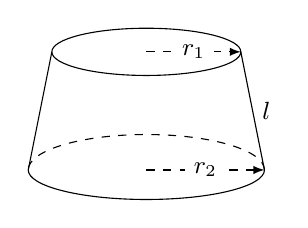
\begin{tikzpicture}[>=latex,every node/.style={font=\small},scale=1.5]
 \draw[->,dashed] (0.5,0) -- (1.5,0) node[midway,fill=white] {$r_2$};
 \draw[->,dashed] (0.5,1) -- (1.3,1) node[midway,fill=white] {$r_1$};
 \draw (-0.3,1) -- (-0.5,0) arc (180:360:1 and 0.25) -- (1.3,1) node[midway,right] {$l$};
 \draw[dashed] (1.5,0) arc (0:180:1 and 0.3);
 \draw (0.5,1) ellipse (0.8 and 0.2);
\end{tikzpicture}}
\noindent To find the total lateral surface area $S$, pick $x$ in
$\lival{a}{b}$ then find the infinitesimal surface area $d\!S$ swept out over
the infinitesimal interval $\ival{x}{x+\dx}$, as in Figure \ref{fig:surfarea}(b).
By the Microstraightness Property, the curve $y=f(x)$ is a straight line segment
of length $\ds$ over that interval, so that the infinitesimal surface is a
\textbf{frustrum}---a right circular cone with the vertex chopped off by a plane
parallel to the base circle. From geometry\footnote{See pp.136-137 in
\textsc{Welchons A.M. and W.R. Krickenberger}, \emph{Solid Geometry}, Boston:
Ginn \& Co., 1936.} you might recall the formula for the lateral surface area of
the frustrum in Figure \ref{fig:frustrum}: $\pi\,(r_1+r_2)\,l$.
Use that formula with $r_1=f(x)$, $r_2=f(x+\dx)=f(x)+\dy$, and
$l=\ds=\sqrt{1 + (f'(x))^2}\,\dx$ (by formula (\ref{eqn:arclength}) in Section
8.3) as in Figure \ref{fig:surfarea}(c), so that $d\!S$ is
\begin{align*}
d\!S ~&=~ \pi\,(f(x) + (f(x)+\dy))\,\sqrt{1 + (f'(x))^2}\,\dx\\
&=~ 2\,\pi\,f(x)\,\sqrt{1 + (f'(x))^2}\,\dx ~+~ \pi\,\sqrt{1 + (f'(x))^2}\,\dy\,\dx\\
&=~ 2\,\pi\,f(x)\,\sqrt{1 + (f'(x))^2}\,\dx ~+~ 0
\end{align*}
since $\dy\,\dx = f'(x)\,(\dx)^2 = 0$.
The surface area $S$ is then the sum of all the areas $d\!S$:

\statethm{thm:surfarea}{The surface area $S$ of the surface of revolution
obtained by revolving the curve $y=f(x) \ge 0$ around the $x$-axis for
$a\le x\le b$ is:
\begin{equation}\label{eqn:surfarea}
S ~=~ \int_a^b d\!S ~=~ \int_a^b 2\,\pi\,f(x)\,\sqrt{1 + (f'(x))^2}~\dx
\end{equation}
For a general curve $y=f(x)$, possibly negative in $\ival{a}{b}$, the
surface area $S$ is:
\begin{equation}\label{eqn:surfareagen}
S ~=~ \int_a^b d\!S ~=~ \int_a^b 2\,\pi\,\abs{y}~\ds ~=~
\int_a^b 2\,\pi\,\Abs{f(x)}\,\sqrt{1 + (f'(x))^2}~\dx
\end{equation}}

\parpic[r]{\begin{tikzpicture}[>=latex,every node/.style={font=\small}]
  \draw[->,black!60,line width=1pt] (0,-1.2) -- (0,1.5) node[above] {$y$};
  \draw[->,black!60,line width=1pt,anchor=base] (0,0) -- (3.5,0) node[right] {$x$}
   node[black,shift={(0,-0.4)}] at (1,0) {$a$}
   node[black,shift={(0,-0.4)}] at (3,0) {$b$};
  \draw[linecolor2,line width=1.5pt] (1,0.6) parabola (3,1.2);
  \draw[linecolor,line width=1.5pt] (1,-0.6) parabola (3,-1.2);
  \draw[black!60] (1,0.1) -- (1,-0.1);
  \draw[black!60] (3,0.1) -- (3,-0.1);
  \fill (1,0.6) circle (2.5pt);
  \fill (3,1.2) circle (2.5pt);
  \fill (1,-0.6) circle (2.5pt);
  \fill (3,-1.2) circle (2.5pt);
  \node[left] at (2.3,1.1) {$y=\Abs{f(x)}$};
  \node[left] at (2.3,-1.1) {$y=f(x)$};
 \end{tikzpicture}}
\noindent Note that formula (\ref{eqn:surfareagen}) holds by symmetry and
formula (\ref{eqn:surfarea}). A curve $y=f(x) <0$ and the curve
$y=\Abs{f(x)}=-f(x)$ are symmetric with respect to the $x$-axis, as in the
figure on the right. Thus, both curves sweep out the same surface of revolution
when revolved around the $x$-axis. This means formula (\ref{eqn:surfareagen})
also holds if $y=f(x)$ changes sign in $\ival{a}{b}$: similar to the area
between two curves, you would split the integral over different subintervals
depending on the sign.

\begin{exmp}
\noindent Show that the surface area of a sphere of radius $r$ is
$4\pi r^2$.\vspace{1mm}
\parpic[r]{\begin{tikzpicture}[>=latex,every node/.style={font=\small}]
 \draw[->,black!60,line width=1pt] (0,-1.3) -- (0,1.5) node[above] {$y$};
 \draw[->,black!60,line width=1pt,anchor=base] (-1.5,0) -- (1.7,0) node[right] {$x$}
  node[black,shift={(0,-0.3)}] at (-1.4,0) {$-r$}
  node[black,shift={(0,-0.3)}] at (1.3,0) {$r$};
 \shade [opacity=0.4,ball color=fillcolor] (0,0) circle (1.2);
 \draw[linecolor,line width=1.5pt] (1.2,0) arc (0:180:1.2);
 \fill (-1.2,0) circle (2.5pt);
 \fill (1.2,0) circle (2.5pt);
 \node[right] at (1,1) {$y=\sqrt{r^2-x^2}$};
\end{tikzpicture}}
\par\noindent\emph{Solution:} Use the circle $x^2+y^2=r^2$. The upper half of
that circle is the curve $y=f(x)=\sqrt{r^2-x^2}$ over the
interval $\ival{-r}{r}$, as in the figure on the right. Revolving that curve
around the $x$-axis produces a sphere of radius $r$, whose surface area $S$ is:
\begin{align*}
S ~&=~ \int_{-r}^r 2\,\pi\,f(x)\,\sqrt{1 + (f'(x))^2}~\dx\\
&=~ \int_{-r}^r 2\,\pi\,\sqrt{r^2-x^2}\,\sqrt{1 + \left(\frac{-x}{\sqrt{r^2-x^2}}\right)^2}~\dx\\
&=~ \int_{-r}^r 2\,\pi\,\cancel{\sqrt{r^2-x^2}}\,\sqrt{\frac{r^2}{\cancel{r^2-x^2}}}~\dx\\
&=~ 2\,\pi\,rx~\Biggr|_{-r}^r ~=~ 4\,\pi r^2 \quad\checkmark
\end{align*}
\end{exmp}
\divider
\vspace{2mm}

A similar derivation using a frustrum yields the surface area $S$ of the surface
of revolution obtained by revolving a curve $y=f(x)$ around the $y$-axis, for
$0\le a\le x\le b$:
\begin{equation}\label{eqn:surfareageny}
S ~=~ \int_a^b d\!S ~=~ \int_a^b 2\,\pi\,\abs{x}~\ds ~=~
\int_a^b 2\,\pi\,x\,\sqrt{1 + (f'(x))^2}~\dx
\end{equation}
\newpage
Now suppose you revolve the region between a curve $y=f(x)\ge 0$ and the
$x$-axis around the $x$-axis, for $a\le x\le b$ (see Figure
\ref{fig:solidvolume}(a)). This produces a \textbf{solid of revolution}
in three dimensions, as in Figure
\ref{fig:solidvolume}(b).\index{solid of revolution} Notice that this solid
consists of the surface of revolution as before along with its interior. 

\begin{figure}[ht]
 \centering
 \subfloat[][\enskip Revolve region around $x$-axis]{
 \begin{tikzpicture}[>=latex,every node/.style={font=\small}]
  \fill[fill=fillcolor] (1,0) -- (1,0.6) parabola (3,1.2) -- (3,0) -- cycle;
  \draw (1,0) -- (1,0.6);
  \draw (3,0) -- (3,1.2);
  \draw[->,black!60,line width=1pt] (0,-1.2) -- (0,1.5) node[above] {$y$};
  \draw[->,black!60,line width=1pt,anchor=base] (0,0) -- (4,0) node[right] {$x$}
   node[black,shift={(0,-0.4)}] at (1,0) {$a$}
   node[black,shift={(0,-0.4)}] at (3,0) {$b$};
  \draw[linecolor,line width=1.5pt] (1,0.6) parabola (3,1.2);
  \draw[black!60] (1,0) -- (1,-0.1);
  \draw[black!60] (3,0) -- (3,-0.1);
  \fill (1,0.6) circle (2.5pt);
  \fill (3,1.2) circle (2.5pt);
  \node[left] at (2.3,1.2) {$y=f(x)$};
  \path (-0.75,0) -- (4.75,0);
  \draw[->] (0.5,0.2) arc (20:340:0.1 and 0.4);
 \end{tikzpicture}}
 \quad
 \subfloat[][\enskip Solid]{
 \begin{tikzpicture}[>=latex,every node/.style={font=\small}]
  \path[name path=ctop] (1,0.6) parabola (3,1.2);
  \path[name path=cbot] (1,-0.6) parabola (3,-1.2);
  \path[name path=xdx] (2,-1.1) rectangle (2.2,1.1);
  \path [name intersections={of=ctop and xdx}];
  \coordinate (A)  at (intersection-1);
  \coordinate (B)  at (intersection-2);
  \path [name intersections={of=cbot and xdx}];
  \coordinate (C)  at (intersection-1);
  \coordinate (D)  at (intersection-2);
  \shadedraw[top color=insideo,bottom color=insideo,middle color=insidei]
   (A) -- (B) arc (90:270:0.3 and 0.815) -- (D) -- (C) arc (270:90:0.3 and 0.75);
  \draw[dashed] (D) arc(-90:90:0.24 and 0.815);
  \draw[dashed] (C) arc(-90:90:0.24 and 0.75);
  \shade [top color=insideo,bottom color=insideo,middle color=insidei]
   (1,0.6) arc (90:270:0.2 and 0.6) --
   (1,-0.6) parabola (3,-1.2) arc (270:90:0.3 and 1.2) parabola[bend at end] (1,0.6);
  \fill[black!30] (B) arc(90:270:0.3 and 0.815) -- (D) arc(270:450:0.24 and 0.815);
  \fill[black!20] (3,1.2) arc (90:450:0.3 and 1.2);
  \draw (1,-0.6) parabola (3,-1.2);
  \draw[->,black!60,line width=1pt] (0,-1.2) -- (0,1.5) node[above] {$y$};
  \draw[->,black!60,line width=1pt,anchor=base] (0,0) -- (4,0) node[right] {$x$}
   node[black,shift={(0,-0.4)}] at (1,0) {$a$}
   node[black,shift={(0,-0.4)}] at (2.05,0) {$x$}
   node[black,shift={(0,-0.4)}] at (3,0) {$b$};
  \draw (A) -- (B) arc (90:270:0.3 and 0.815) -- (D) -- (C) arc (270:90:0.3 and 0.75);
  \draw[dashed] (D) arc(-90:90:0.24 and 0.815);
  \draw[dashed] (C) arc(-90:90:0.24 and 0.75);
  \draw (1,0.6) arc (90:270:0.2 and 0.6);
  \draw[dashed] (1,0.6) arc (90:-90:0.2 and 0.6);
  \draw (3,1.2) arc (90:450:0.3 and 1.2);
  \draw[linecolor,line width=1.5pt] (1,0.6) parabola (3,1.2);
  \draw[black!60] (1,0.1) -- (1,-0.1);
  \draw[black!60] (3,0.1) -- (3,-0.1);
  \draw[black!60] (2.05,0.1) -- (2.05,-0.1);
  \fill (1,0.6) circle (2.5pt);
  \fill (3,1.2) circle (2.5pt);
  \node[left] at (2.3,1.2) {$y=f(x)$};
 \end{tikzpicture}}
 \quad
 \subfloat[][\enskip Infinitesimal strip]{
 \begin{tikzpicture}[>=latex,every node/.style={font=\small}]
  \draw[->|] (0.7,0) -- (0.7,1.5) node[fill=white,midway] {$f(x)$};
  \draw[->|] (2.2,0) -- (2.2,2.1) node[fill=white,pos=0.3,xshift=0.3cm] {$f(x+\dx)$};
  \fill[black!30] (1.05,0) -- (1.05,1.5) -- (1.5,1.5) -- (1.5,0) -- cycle;
  \draw[dashed] (1.05,1.5) -- (1.5,1.5);
  \draw (1.05,0) -- (1.05,1.5);
  \draw (1.5,0) -- (1.5,2.1);
  \draw[<->,black!60,line width=1pt] (0,2.2) node[above] {$y$} |- (3,0) node[right] {$x$};
  \draw[linecolor,line width=1.5pt] (1.05,1.5) -- (1.5,2.1) node[black,sloped,midway,above] {$\ds$};  
  \node at (1.275,-0.2) {$\dx$};
  \draw[->|] (0.8,-0.2) -- (1.05,-0.2);
  \draw[->|] (1.75,-0.2) -- (1.5,-0.2);
  \draw[->|] (1.8,1.2) -- (1.8,1.5);
  \draw[->|] (1.8,2.4) -- (1.8,2.1);
  \node at (1.8,1.8) {$\dy$};
 \end{tikzpicture}}
 \caption[]{\enskip Solid of revolution over $\ival{a}{b}$ with volume area $V$}
 \label{fig:solidvolume}
\end{figure}

The goal is to find the volume $V$ of this solid. The idea is to divide the
solid into slices, like a loaf of bread. First, the
infinitesimal volume $d\!V$ of the frustrum swept out by a strip of
infinitesimal width $\dx$ at $x$ in $\lival{a}{b}$---shown in Figure
\ref{fig:solidvolume}(c)---is needed. By the Microstraightness Property the
curve $y=f(x)$ is a straight line of length $\ds$ over the interval
$\ival{x}{x+\dx}$. There is thus a right triangle at the top of the
strip---unshaded in Figure \ref{fig:solidvolume}(c)---whose area $A$ is zero:
$A = \tfrac{1}{2} (\dy)(\dx) = \tfrac{1}{2} f'(x) (\dx)^2 = 0$.

\piccaption[]{\label{fig:discmethod}}\parpic[r]{
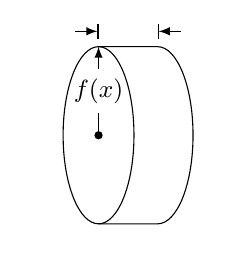
\begin{tikzpicture}[>=latex,every node/.style={font=\small},scale=1.5]
 \draw[->] (0,0) -- (0,0.75) node[midway,fill=white] {$f(x)$};
 \draw (0,0) ellipse (0.3 and 0.75);
 \draw (0,-0.75) -- (0.5,-0.75) arc (-90:90:0.3 and 0.75) -- (0,0.75) node[midway,above] {$\dx$};
 \fill (0,0) circle (1pt);
 \draw[->|] (-0.2,0.88) -- (0,0.88);
 \draw[->|] (0.7,0.88) -- (0.5,0.88);
 \path (-0.6,0) -- (1,0);
\end{tikzpicture}}
That triangle thus contributes no volume when revolved around the
$x$-axis: the volume $d\!V$ swept out by that strip all comes from the shaded
rectangle of height $f(x)$ and width $\dx$. That rectangle sweeps out a right
circular cylinder of radius $f(x)$ and height $\dx$ (see Figure
\ref{fig:discmethod}). The volume of a right circular cylinder of radius $r$ and
height $h$ is defined as the area of the base circle times the height:
$\pi r^2h$. Hence,
\[
d\!V ~=~ \pi\,(f(x))^2\;\dx ~~.
\]
The total volume $V$ of the solid is then the sum of all those infinitesimal
volumes $d\!V$:\index{disc method}\index{solid of revolution!disc method}

\statethm{thm:volumedisc}{The volume $V$ of the solid of revolution
obtained by revolving the region between the curve $y=f(x)$ and the $x$-axis
around the $x$-axis for $a\le x\le b$ is:
\begin{equation}\label{eqn:volumedisc}
V ~=~ \int_a^b d\!V ~=~ \int_a^b \pi\,(f(x))^2~\dx
\end{equation}}
\noindent This method for finding the volume is called the \textbf{disc method},
since the cylinder of volume $d\!V$ resembles a disc. Think of the discs as
being similar to infinitesimally thin slices of a loaf of bread. Notice that
absolute values are not needed in formula (\ref{eqn:volumedisc}) since $f(x)$ is
squared, so the formula holds even when $f(x)$ is negative.
\newpage
\begin{exmp}
\noindent Show that the volume of a sphere of radius $r$ is
$\frac{4}{3} \pi r^3$.\vspace{0.5mm}
\parpic[r]{\begin{tikzpicture}[>=latex,every node/.style={font=\small}]
 \draw[->,black!60,line width=1pt] (0,-1.3) -- (0,1.5) node[above] {$y$};
 \draw[->,black!60,line width=1pt,anchor=base] (-1.5,0) -- (1.7,0) node[right] {$x$}
  node[black,shift={(0,-0.3)}] at (-1.4,0) {$-r$}
  node[black,shift={(0,-0.3)}] at (1.3,0) {$r$};
 \shade [opacity=0.4,ball color=fillcolor] (0,0) circle (1.2);
 \draw[linecolor,line width=1.5pt] (1.2,0) arc (0:180:1.2);
 \fill (-1.2,0) circle (2.5pt);
 \fill (1.2,0) circle (2.5pt);
 \node[right] at (1,1) {$y=\sqrt{r^2-x^2}$};
\end{tikzpicture}}
\par\noindent\emph{Solution:} Use the circle $x^2+y^2=r^2$. Revolve the region
between the upper half of the circle $y=f(x)=\sqrt{r^2-x^2}$ and the $x$-axis
around the $x$-axis over the interval $\ival{-r}{r}$, as in the figure on the
right. The solid of revolution swept out is a sphere of radius $r$, whose volume
$V$ is:
\begin{align*}
V ~&=~ \int_{-r}^r \pi\,(f(x))^2~\dx ~=~
       \int_{-r}^r \pi\,(r^2-x^2)~\dx ~=~
       \pi\,r^2 x ~-~ \frac{1}{3} \pi x^3~\Biggr|_{-r}^r\\
&=~    \left(\pi\,r^3 - \frac{1}{3} \pi r^3\right) ~-~ \left(-\pi\,r^3 + \frac{1}{3} \pi r^3\right)
~=~ \frac{4}{3}\,\pi r^3 \quad\checkmark
\end{align*}
\end{exmp}
\divider
\vspace{2mm}

Instead of memorizing formula (\ref{eqn:volumedisc}), try to remember the more
generic approach of revolving an infinitesimal rectangular strip around an axis,
which might not be the $x$-axis. The idea is to find the radius $r$ and height
$h$---typically $\dx$ or $\dy$---of the disc swept out by that strip, so that
the disc's volume is $d\!V = \pi r^2 h$. Then integrate $d\!V$ over the
appropriate interval to find the volume $V$ of the entire solid.

\begin{exmp}
\noindent Suppose the region bounded by the curve $y=x^2$ and the $x$-axis
for $0 \le x \le 1$ is revolved around the line $x=1$. Find the
volume of the resulting solid of revolution.\vspace{0.5mm}
\parpic[r]{\begin{tikzpicture}[>=latex,every node/.style={font=\small}]
 \fill[fillcolor] (0,0) parabola (1.5,1.5) -- (1.5,0) -- cycle;
 \draw[linecolor,line width=1.5pt] (0,0) parabola (1.5,1.5);
 \draw (1.5,1.5) parabola[bend at end] (3,0);
 \draw[dashed] (1.5,0) -- (1.5,1.9) node[above] {$x=1$};
 \draw[<->,black!60,line width=1pt,anchor=base] (0,2) node[above] {$y$} |- (3.5,0) node[right] {$x$}
  node[black,shift={(0,-0.4)}] at (0,0) {$0$}
  node[black,shift={(0,-0.4)}] at (0.7,0) {$x$}
  node[black,shift={(0,-0.4)}] at (1.5,0) {$1$};
 \fill (0,0) circle (2.5pt);
 \fill (1.5,1.5) circle (2.5pt);
 \node[left] at (1.4,1.3) {$y=x^2$};
 \draw (0.7,0.33) -- (1.5,0.33) node[pos=0.6,above,yshift=-0.05cm] {$r$} -- (1.5,0.2)
  node[midway,right] {$h$} -- (0.7,0.2) -- cycle;
 \draw[black!60] (0.7,0.1) -- (0.7,-0.1);
 \draw[black!60] (-0.1,0.26) -- (0.1,0.26);
 \node[left] at (-0.1,0.26) {$x^2=y$};
 \draw[black!60] (-0.1,1.5) -- (0.1,1.5);
 \node[left] at (-0.1,1.5) {$1$};
\end{tikzpicture}}
\par\noindent\emph{Solution:} The region is shaded in the figure on the right.
Since the region is revolved around a vertical axis, the disc method
will use discs with height $\dy$, not $\dx$.
At a point $x$ in $\ival{0}{1}$ go up to the curve $y=x^2$ and draw a horizontal
rectangular strip to the line $x=1$, as shown in the figure. Let
$h=\dy$ and revolve that strip around the line $x=1$, producing a disc of radius
$r-1-x$ and height $h=\dy$. Since $y=x^2$ implies $x=\sqrt{y}$, the volume
$d\!V$ of that disc is
\[
d\!V ~=~ \pi\,r^2 h ~=~ \pi\,(1-x)^2~\dy ~=~ \pi\,(1-\sqrt{y})^2~\dy ~=~
\pi\,(1 - 2\sqrt{y} + y)~\dy ~.
\]
The volume $V$ of the entire solid is then the sum of those volumes $d\!V$ along
the $y$-axis for $0\le y\le 1$:
\[
V ~=~ \int_0^1 d\!V ~=~ \int_0^1 \pi\,(1 - 2\sqrt{y} + y)~\dy ~=~
\pi\,\left(y - \frac{4}{3}y^{3/2} + \frac{1}{2}y^2 \right)~\Biggr|_0^1 ~=~
\pi\,\left(1 - \frac{4}{3} + \frac{1}{2}\right) ~=~ \frac{\pi}{6}
\]
\end{exmp}
\divider
\vspace{2mm}

\parpic[r]{\begin{tikzpicture}[>=latex,every node/.style={font=\small}]
 \fill[fillcolor] (1,0) -- (1,0.7) parabola (2,1.2) -- (2,0) -- cycle;
 \draw (1,0) -- (1,0.7);
 \draw (2,0) -- (2,1.2);
 \draw[->,black!60,line width=1pt] (0,0) -- (0,1.7) node[above] {$y$};
 \draw[->,black!60,line width=1pt,anchor=base] (-2.2,0) -- (2.5,0) node[right] {$x$}
  node[black,shift={(0,-0.4)}] at (1,0) {$a$}
  node[black,shift={(0,-0.4)}] at (-1,0) {$-a$}
  node[black,shift={(0,-0.4)}] at (0,0) {$0$}
  node[black,shift={(0,-0.4)}] at (2,0) {$b$}
  node[black,shift={(0,-0.4)}] at (-2,0) {$-b$};
 \draw[linecolor,line width=1.5pt] (1,0.7) parabola (2,1.2);
 \fill (1,0.7) circle (2.5pt);
 \fill (2,1.2) circle (2.5pt);
 \draw[black!60] (-1,0.1) -- (-1,-0.1);
 \draw[black!60] (-2,0.1) -- (-2,-0.1);
 \draw[->] (0.5,0.5) arc (0:320:0.5 and 0.2);
 \node[left] at (1.7,1.1) {$y=f(x)$};
\end{tikzpicture}}
The \textbf{shell method} can be used for finding the volume of a solid with a
``hole'' in the middle, as in the solid of revolution produced by revolving the
shaded region in the figure on the right around the $y$-axis. The hole in the
solid between $x=-a$ and $x=a$ is a result of the gap between the $y$-axis and
the region.\index{shell method}
\newpage
To find the volume $V$ of that solid, at a point $x$ in $\lival{a}{b}$ form an
infinitesimal strip of width $\dx$ from the $x$-axis up to the curve $y=f(x)$,
as in Figure \ref{fig:shellmethod}(a).

\begin{figure}[ht]
 \centering
 \subfloat[][\enskip Revolve region around $y$-axis]{
 \begin{tikzpicture}[>=latex,every node/.style={font=\small}]
  \fill[fillcolor] (1,0) -- (1,0.7) parabola (2,1.2) -- (2,0) -- cycle;
  \draw (1,0) -- (1,0.7);
  \draw (2,0) -- (2,1.2);
  \fill[pattern=north west lines] (1.5,0) -- (1.5,0.8) -- (1.7,0.95) -- (1.7,0);
  \draw[<->,black!60,line width=1pt,anchor=base] (0,1.7) node[above] {$y$} |- (2.5,0)
   node[right] {$x$}
   node[black,shift={(0,-0.4)}] at (0,0) {$0$}
   node[black,shift={(0,-0.4)}] at (1,0) {$a$}
   node[black,shift={(0,-0.4)}] at (1.5,0) {$x$}
   node[black,shift={(0,-0.4)}] at (2,0) {$b$};
  \draw (1.5,0) -- (1.5,0.8);
  \draw (1.7,0) -- (1.7,0.95);
  \draw[linecolor,line width=1.5pt] (1,0.7) parabola (2,1.2);
  \fill (1,0.7) circle (2.5pt);
  \fill (2,1.2) circle (2.5pt);
  \node[left] at (1.7,1.1) {$y=f(x)$};
  \path (-1.3,0) -- (3.7,0);
 \end{tikzpicture}}
 \quad
 \subfloat[][\enskip Infinitesimal strip]{
 \begin{tikzpicture}[>=latex,every node/.style={font=\small}]
  \draw[->|] (0.7,0) -- (0.7,1.5) node[fill=white,midway] {$f(x)$};
  \draw[->|] (2.2,0) -- (2.2,2.1) node[fill=white,pos=0.3,xshift=0.2cm] {$f(x+\dx)$};
  \fill[black!30] (1.05,0) -- (1.05,1.5) -- (1.5,1.5) -- (1.5,0) -- cycle;
  \draw[dashed] (1.05,1.5) -- (1.5,1.5);
  \draw (1.05,0) -- (1.05,1.5);
  \draw (1.5,0) -- (1.5,2.1);
  \draw[<->,black!60,line width=1pt] (0,2.2) node[above] {$y$} |- (3,0) node[right] {$x$};
  \draw[linecolor,line width=1.5pt] (1.05,1.5) -- (1.5,2.1) node[black,sloped,midway,above] {$\ds$};  
  \node at (1.275,-0.2) {$\dx$};
  \draw[->|] (0.8,-0.2) -- (1.05,-0.2);
  \draw[->|] (1.75,-0.2) -- (1.5,-0.2);
  \draw[->|] (1.8,1.2) -- (1.8,1.5);
  \draw[->|] (1.8,2.4) -- (1.8,2.1);
  \node at (1.8,1.8) {$\dy$};
 \end{tikzpicture}}
 \quad
 \subfloat[][\enskip Cylindrical shell]{
 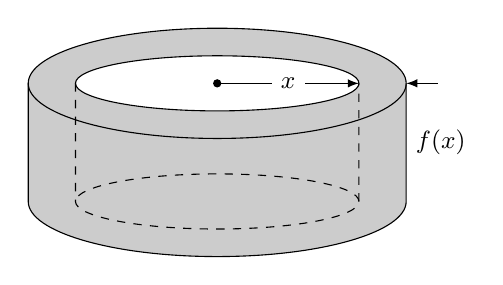
\begin{tikzpicture}[>=latex,every node/.style={font=\small}]
  \fill[black!20] (2.4,1.5) arc (0:180:2.4 and 0.7) -- (-2.4,0) arc (180:360:2.4 and 0.7) -- cycle;
  \filldraw[fill=white,draw=black] (0,1.5) ellipse (1.8 and 0.35);
  \draw (0,1.5) ellipse (2.4 and 0.7);
  \draw (-2.4,1.5) -- (-2.4,0) arc (180:360:2.4 and 0.7) -- (2.4,1.5) node[midway,right] {$f(x)$};
  \draw[dashed] (-1.8,1.5) -- (-1.8,0) arc (180:360:1.8 and 0.35) -- (1.8,1.5);
  \draw[dashed] (1.8,0) arc (0:180:1.8 and 0.35);
  \draw[->] (0,1.5) -- (1.8,1.5) node[midway,fill=white] {$x$};
  \draw[->] (2.8,1.5) -- (2.4,1.5);
  \node at (2.1,1.5) {$\dx$};
  \fill (0,1.5) circle (1.5pt);
 \end{tikzpicture}}
 \caption[]{\enskip Shell method}
 \label{fig:shellmethod}
\end{figure}

Just like the strip in the disc method, the right triangle at the top of
this strip---as in Figure \ref{fig:shellmethod}(b)---has zero area and thus does
not contribute to the volume $d\!V$ of the right circular cylindrical shell
swept out by the strip, shown in Figure \ref{fig:shellmethod}(c). The volume of
that shell is just the volume of the ``outer'' cylinder of radius $x+\dx$ minus
the volume of the ``inner'' cylinder of radius $x$, both with height $f(x)$:
\begin{align*}
d\!V ~&=~ \pi\,(x+\dx)^2\,f(x) ~-~ \pi\,x^2\,f(x)\\[-6pt]
&=~ \cancel{\pi\,x^2\,f(x)} ~+~ 2\,\pi\,x\,f(x)\,\dx ~+~
    \pi\,\cancelto{0}{(\dx)^2}\,f(x) ~-~ \cancel{\pi\,x^2\,f(x)}\\
&=~ 2\,\pi\,x\,f(x)\,\dx
\end{align*}
The volume $V$ of the entire solid is then the sum of those volumes $d\!V$,
using an absolute value to handle any sign for $f(x)$:

\statethm{thm:volumeshell}{The volume $V$ of the solid of revolution
obtained by revolving the region between the curve $y=f(x)$ and the $x$-axis
around the $y$-axis for $0\le a\le x\le b$ is:
\begin{equation}\label{eqn:volumeshell}
V ~=~ \int_a^b d\!V ~=~ \int_a^b 2\,\pi\,x\,\Abs{f(x)}~\dx
\end{equation}}

\begin{exmp}
\noindent Suppose the region bounded by the curve $y=x^2$ and the $x$-axis
for $0 \le x \le 1$ is revolved around the $y$-axis. Find the
volume of the resulting solid of revolution.\vspace{0.5mm}
\parpic[r]{\begin{tikzpicture}[>=latex,every node/.style={font=\small}]
 \fill[fillcolor] (0,0) parabola (1.5,1.5) -- (1.5,0) -- cycle;
 \draw (1.5,0) -- (1.5,1.5);
 \draw[linecolor,line width=1.5pt] (0,0) parabola (1.5,1.5);
 \draw[black!60] (1,0.1) -- (1,-0.1);
 \draw (1,0) -- (1,0.66)  -- (1.15,0.66) -- (1.15,0);
 \draw[<->,black!60,line width=1pt,anchor=base] (0,2) node[above] {$y$} |- (2.2,0) node[right] {$x$}
  node[black,shift={(0,-0.4)}] at (0,0) {$0$}
  node[black,shift={(0,-0.4)}] at (1,0) {$x$}
  node[black,shift={(0,-0.4)}] at (1.5,0) {$1$};
 \fill (0,0) circle (2.5pt);
 \fill (1.5,1.5) circle (2.5pt);
 \node[left] at (1.4,1.3) {$y=x^2$};
 \draw[black!60] (-0.1,1.5) -- (0.1,1.5);
 \node[left] at (-0.1,1.5) {$1$};
\end{tikzpicture}}
\par\noindent\emph{Solution:} The region is shaded in the figure on the right.
The vertical strip at $x$ in $\lival{0}{1}$ with infinitesimal width $\dx$ and
height $\Abs{f(x)}=f(x)$ is shown in the figure. That strip produces the shell
with volume $d\!V$ in formula (\ref{eqn:volumeshell}), so by the shell method
the volume $V$ of the solid of revolution is:
\[
V ~=~ \int_0^1 d\!V ~=~ \int_0^1 2\,\pi\,x\,\Abs{f(x)}~\dx ~=~
\int_0^1 2\,\pi\,x\,\cdot\,x^2~\dx ~=~ \frac{\pi}{2}\,x^4~\Biggr|_0^1 ~=~
\frac{\pi}{2}
\]
\end{exmp}
\divider
\newpage
The volume $d\!V$ in formula (\ref{eqn:volumeshell}) can be generalized to
$d\!V = 2 \pi r h w$, where $r$ is the distance from the axis of
revolution to a generic vertical strip of infinitesimal width $w$ in the region,
and $h$ is the height of the strip.
\begin{exmp}\label{exmp:shell1}
\noindent Suppose the region bounded by the curves $y=x^2$ and $y=x$ is revolved
around the $y$-axis. Find the volume of the resulting solid of
revolution.\vspace{0.5mm}
\parpic[r]{\begin{tikzpicture}[>=latex,every node/.style={font=\small}]
 \fill[fillcolor] (0,0) parabola (1.5,1.5) -- cycle;
 \draw[linecolor,line width=1.5pt] (0,0) parabola (1.5,1.5);
 \draw[linecolor,line width=1.5pt] (0,0) -- (1.5,1.5);
 \draw[black!60] (0.7,0.1) -- (0.7,-0.1);
 \draw (0.7,0.33)  -- (0.7,0.7) -- (0.8,0.7) -- (0.8,0.33) -- cycle;
 \draw[<->,black!60,line width=1pt,anchor=base] (0,1.9) node[above] {$y$} |- (2.2,0) node[right] {$x$}
  node[black,shift={(0,-0.4)}] at (0,0) {$0$}
  node[black,shift={(0,-0.4)}] at (0.7,0) {$x$}
  node[black,shift={(0,-0.4)}] at (1.5,0) {$1$};
 \fill (0,0) circle (2.5pt);
 \fill (1.5,1.5) circle (2.5pt);
 \node[left] at (1.2,1.3) {$y=x$};
 \node[right] at (1.1,0.6) {$y=x^2$};
 \draw[black!60] (-0.1,1.5) -- (0.1,1.5);
 \node[left] at (-0.1,1.5) {$1$};
\end{tikzpicture}}
\par\noindent\emph{Solution:} The region is shaded in the figure on the right,
along with a vertical strip with infinitesimal width $w=\dx$ at the distance
$r=x$ from the $y$-axis in the region and height $h=x-x^2$. That strip produces
the shell with volume $d\!V=2\pi rhw=2\pi x(x-x^2)\,\dx$, so that the volume $V$
of the solid of revolution is:
\[
V ~=~ \int_0^1 d\!V ~=~ \int_0^1 2\,\pi\,x\,(x-x^2)~\dx ~=~
\frac{2\pi}{3}\,x^3 ~-~ \frac{\pi}{2}\,x^4~\Biggr|_0^1 ~=~
\frac{\pi}{6}
\]
\end{exmp}
\divider
\vspace{2mm}
\startexercises\label{sec8dot4}
{\small
\probs{A}
\par\noindent For Exercises 1-3, find the surface area of the surface of
revolution produced by revolving the given curve around the $x$-axis for the
given interval.
\begin{enumerate}[\bfseries 1.]
\begin{multicols}{3}
 \item $y = \sqrt{4 - x^2}~$ for $~1 \le x \le 2\vphantom{\frac{x^3}{6}}$
 \item $y = \cosh\,x~$ for $~0 \le x \le 1\vphantom{\frac{x^3}{6}}$
 \item $y = \frac{x^3}{6} + \frac{1}{2x}~$ for $~1 \le x \le 3$
\end{multicols}
\suspend{enumerate}
\par\noindent For Exercises 4-6, find the volume of the solid of revolution
produced by revolving the region between the given curve and the $x$-axis around
the $x$-axis for the given interval.
\resume{enumerate}[{[\bfseries 1.]}]
\begin{multicols}{3}
 \item $y = x^3~$ for $~0 \le x \le 1$
 \item $y = \sin\,x~$ for $~0 \le x \le \pi$
 \item $y = \sqrt{x}~$ for $~0 \le x \le 1$
\end{multicols}
\suspend{enumerate}
\par\noindent For Exercises 7-9, find the volume of the solid of revolution
produced by revolving the region between the given curve and the $x$-axis around
the $y$-axis for the given interval.
\resume{enumerate}[{[\bfseries 1.]}]
\begin{multicols}{3}
 \item $y = \sin\,(x^2)~$ for $~0 \le x \le \sqrt{\pi}$
 \item $y = \sin\,x~$ for $~0 \le x \le \pi$
 \item $y = x^2 - x^3~$ for $~0 \le x \le 1$
\end{multicols}
 \item Revolve the region in Example \ref{exmp:shell1} around the line $x=1$ and
  find the volume of the resulting solid.
 \item\label{exer:ellipsoid} Revolving the ellipse\index{ellipsoid}
  $\frac{x^2}{a^2}+\frac{y^2}{b^2}=1$ around the $x$-axis produces an
  \emph{ellipsoid}, for $a>b>0$. Show that the surface area of the ellipsoid is
  $2\,\pi\,b^2\,\left(1 + \frac{a}{eb}\,\sin^{-1} e\right)$, where $e$ is the
  eccentricity of the ellipse.
 \item Show that the volume inside the ellipsoid from Exercise
  \ref{exer:ellipsoid} is $\frac{4}{3}\,\pi\,a\,b^2$.
 \item Find the surface area and volume of a right circular cone of radius $r$
  and height $h$.
 \item Formulas (\ref{eqn:surfareagen}), (\ref{eqn:volumedisc}) and
  (\ref{eqn:volumeshell}) can be extended to include regions over infinite
  intervals---the integrals in those formulas simply become improper integrals.
  Consider the region between the curve $y=\frac{1}{x}$ and the $x$-axis over
  the interval $\lival{1}{\infty}$. Revolve that region around the $x$-axis.
\begin{enumerate}[\bfseries (a)]
 \item Show that the surface area of the resulting surface of revolution is
  infinite.
 \item Show that the volume of the resulting solid of revolution is $\pi$.
% \item Does the result of part (b) contradict that of part (a)? Explain.
\end{enumerate}
 \item\label{exer:torus} For $0<a<b$, revolving the region inside the circle
  $(x-b)^2+y^2=a^2$ around the $y$-axis produces a donut-shaped solid of
  revolution called a \emph{torus}.\index{torus} Show that the volume of the
  torus is $2\pi^2a^2b$.
 \item Use formula (\ref{eqn:surfareageny}) and symmetry to show that the torus
  from Exercise \ref{exer:torus} has surface area $4\pi^2ab$.
\end{enumerate}}
\newpage
%Begin Section 8.5
\section{Applications in Physics and Statistics}
This chapter concludes with a few applications showing how some familiar
discrete sums can be replaced by integrals, which are essentially
continuous sums.\index{center of gravity}\\

\noindent{\large\textbf{Center of Gravity}}\\

Suppose a thin uniform rod has $n>1$ masses $m_1,\ldots,m_n$
attached, with $m_1$ and $m_n$ at the ends. The \textbf{center of gravity} of
the masses is the point where---due to the Earth's gravity---the rod would be
balanced if a fulcrum were placed there (see Figure \ref{fig:m1m2rod}(a)).
Imagine the rod as part of the $x$-axis and the weights as point masses---with
each mass $m_k$ at $x_k$---and let the center of gravity be at $\bar{x}$, as in
Figure \ref{fig:m1m2rod}(b).

\begin{figure}[ht]
 \centering
 \subfloat[][\enskip Rod balanced on fulcrum]{
 \begin{tikzpicture}[>=latex,every node/.style={font=\small}]
  \filldraw[black] (-0.3,-0.3) -- (0,-0.035) -- (0.3,-0.3) -- cycle;
  \draw[linecolor,line width=1.5pt] (-2,0) -- (2,0);
  \fill (-2,0) circle (4pt);
  \fill (-1,0) circle (4pt);
  \fill (1,0) circle (4pt);
  \fill (2,0) circle (4pt);
  \node[above] at (-2,0.2) {$m_1$};
  \node[above] at (-1,0.2) {$m_2$};
  \node[above] at (0,0.2) {$\cdots$};
  \node[above] at (1,0.2) {$m_{n-1}$};
  \node[above] at (2,0.2) {$m_n$};
 \end{tikzpicture}}
 \qquad\qquad
 \subfloat[][\enskip Masses and $\bar{x}$ on $x$-axis]{
 \begin{tikzpicture}[>=latex,every node/.style={font=\small}]
  \draw[->,black!60,line width=1pt,anchor=base] (-1,0) -- (5,0) node[right] {$x$}
   node[black,shift={(0,-0.4)}] at (0,0) {$x_1$}
   node[black,shift={(0,-0.4)}] at (1,0) {$x_2$}
   node[black,shift={(0,-0.4)}] at (2,0) {$\bar{x}$}
   node[black,shift={(0,-0.4)}] at (3,0) {$x_{n-1}$}
   node[black,shift={(0,-0.4)}] at (4,0) {$x_n$};
  \draw[black!60] (2,0.1) -- (2,-0.1);
  \draw[linecolor,line width=1.5pt] (0,0) -- (4,0);
  \fill (0,0) circle (2.5pt);
  \fill (1,0) circle (2.5pt);
  \fill (3,0) circle (2.5pt);
  \fill (4,0) circle (2.5pt);
  \node[above] at (0,0.1) {$m_1$};
  \node[above] at (1,0.1) {$m_2$};
  \node[above] at (2,0.1) {$\cdots$};
  \node[above] at (3,0.1) {$m_{n-1}$};
  \node[above] at (4,0.1) {$m_n$};
 \end{tikzpicture}}
 \caption[]{\enskip Center of gravity $\bar{x}$ for masses $m_1,\ldots,m_n$}
 \label{fig:m1m2rod}
\end{figure}

The rod is balanced if the masses do not rotate the rod, i.e. the total
\textbf{torque} is zero. Torque is defined here as force times position relative
to $\bar{x}$. Each mass $m_k$ applies a force $m_kg$ to the rod---where $g$ is
the (downward) acceleration due to the Earth's gravity---at position
$(x_x-\bar{x})$ relative to $\bar{x}$. The total torque is thus zero if
\[
(m_1g)\,(x_1-\bar{x}) ~+~ (m_2g)\,(x_2-\bar{x}) ~+~ \cdots ~+~
(m_ng)\,(x_n-\bar{x}) ~=~ 0
\]
so that solving for $\bar{x}$ yields:\index{torque}\index{moment}
\begin{equation}\label{eqn:cogdiscrete}
\bar{x} ~=~ \frac{m_1gx_1 + \cdots +  m_ngx_n}{m_1g + \cdots + m_ng} ~=~
            \frac{m_1x_1 + \cdots + m_nx_n}{m_1 + \cdots + m_n} ~=~
            \frac{\sum_{k=1}^n \;m_kx_k}{\sum_{k=1}^n \;m_k}
\end{equation}
Each quantity $m_kx_k$ is called the \textbf{moment} of the mass $m_k$. Thus,
$\bar{x}$ is the sum of the moments divided by the total mass. This idea can be
extended to regions in the $xy$-plane, using an integral of a continuum of
moments instead of a finite sum. The \textbf{center of gravity} of a
planar region is defined as the point such that any force along a line through
that point produces no rotation of the region about that line.\footnote{For a
proof that such a point exists, see p.206 in \textsc{Brown, F.L.},
\emph{Engineering Mechanics}, 2nd ed., New York: John Wiley \& Sons, Inc., 1942.
Some texts use the terms ``center of mass'' or ``centroid'' instead of ``center
of gravity,'' and there are differences in the meanings. However, for the
situation presented here, where the gravitational field is assumed to have
constant magnitude and direction throughout the region, they all mean the same
thing.} There should thus be zero torque in both the $x$ and $y$ directions, so
the idea is to apply formula (\ref{eqn:cogdiscrete}) in both directions
to obtain the region's center of gravity $(\bar{x},\bar{y})$.
\newpage
A region can be thought of as a \textbf{lamina}---a thin plate with uniform
density. Take the area of the region as its mass, which makes sense
given the uniform density. For the region between two curves
$y=f_1(x)$ and $y=f_2(x)$ over $\ival{a}{b}$, with $f_1(x) \ge f_2(x)$, take a
vertical slice of width $\dx$ at some $x$, as in Figure \ref{fig:cogregion}(a).
By the same arguments used in Section 8.4, all the area from that strip comes
from the rectangle of height $f_1(x)-f_2(x)$ and width $\dx$ (see the shaded
rectangle in Figure \ref{fig:cogregion}(b)).\index{lamina}

\begin{figure}[ht]
 \centering
 \subfloat[][\enskip Region between $y=f_1(x)$ and $y=f_2(x)$]{
 \begin{tikzpicture}[>=latex,every node/.style={font=\small}]
  \fill[fillcolor] (1,0.8) -- (1,1.5) parabola (2,2) -- (2,0.6) -- cycle;
  \draw (1,0.8) -- (1,1.5);
  \draw (2,0.6) -- (2,2);
  \fill[pattern=north west lines] (1.5,0.7) -- (1.5,1.6) -- (1.7,1.75) -- (1.7,0.65);
  \draw[<->,black!60,line width=1pt,anchor=base] (0,2.1) node[above] {$y$} |- (3,0)
   node[right] {$x$}
   node[black,shift={(0,-0.4)}] at (0,0) {$0$}
   node[black,shift={(0,-0.4)}] at (1,0) {$a$}
   node[black,shift={(0,-0.4)}] at (1.5,0) {$x$}
   node[black,shift={(0,-0.4)}] at (2,0) {$b$};
  \draw (1.5,0.7) -- (1.5,1.6);
  \draw (1.7,0.65) -- (1.7,1.75);
  \draw[linecolor,line width=1.5pt] (1,1.5) parabola (2,2);
  \draw[linecolor,line width=1.5pt] (1,0.8) -- (2,0.6);
  \fill (1,1.5) circle (2.5pt);
  \fill (2,2) circle (2.5pt);
  \fill (1,0.8) circle (2.5pt);
  \fill (2,0.6) circle (2.5pt);
  \node[left] at (1.7,1.9) {$y=f_1(x)$};
  \node[left] at (1.7,0.4) {$y=f_2(x)$};
  \draw[black!60] (1,0.1) -- (1,-0.1);
  \draw[black!60] (1.5,0.1) -- (1.5,-0.1);
  \draw[black!60] (2,0.1) -- (2,-0.1);
  \path (-1.8,0) -- (4.5,0);
 \end{tikzpicture}}
 \qquad
 \subfloat[][\enskip Infinitesimal strip over $\ival{x}{x+\dx}$]{
 \begin{tikzpicture}[>=latex,every node/.style={font=\small}]
  \draw[|<->|] (0.7,0.4) -- (0.7,1.5) node[fill=white,midway,xshift=-0.5cm] {$f_1(x)-f_2(x)$};
  \fill[black!30] (1.05,0.4) -- (1.05,1.5) -- (1.5,1.5) -- (1.5,0.4) -- cycle;
  \draw[dashed] (1.05,1.5) -- (1.5,1.5);
  \draw[dashed] (1.05,0.4) -- (1.5,0.4);
  \draw (1.05,0.4) -- (1.05,1.5);
  \draw (1.5,0.2) -- (1.5,2.1);
  \draw[<->,black!60,line width=1pt] (-1,2.1) node[above] {$y$} |- (3,0) node[right] {$x$};
  \draw[linecolor,line width=1.5pt] (1.05,1.5) -- (1.5,2.1) node[black,sloped,midway,above] {$\ds$};  
  \draw[linecolor,line width=1.5pt] (1.05,0.4) -- (1.5,0.2);
  \node at (1.275,-0.2) {$\dx$};
  \draw[->|] (0.8,-0.2) -- (1.05,-0.2);
  \draw[->|] (1.75,-0.2) -- (1.5,-0.2);
  \draw[->|] (1.8,1.2) -- (1.8,1.5);
  \draw[->|] (1.8,2.4) -- (1.8,2.1);
  \node at (1.8,1.8) {$\dy$};
  \fill (1.275,0.95) circle (1.5pt);
  \draw[->] (2.1,0.95) -- (1.35,0.95);
  \node[right] at (2.1,0.95) {$(x+\tfrac{1}{2}\dx,\tfrac{1}{2}(f_1(x)+f_2(x)))$};
  \path (-1,0) -- (6,0);
 \end{tikzpicture}}
 \caption[]{\enskip Center of gravity of a region}
 \label{fig:cogregion}
\end{figure}

By the assumption of uniform density, the center of gravity of that rectangle is
clearly its geometric center, whose coordinates are\index{moment}
$\left(x+\frac{1}{2}\dx,\frac{1}{2}(f_1(x)+f_2(x))\right)$. The entire mass of
the strip can be treated as if it is concentrated at that point. The
\textbf{moment} $m_x$ of the strip about the $x$-axis is its mass times the
position of its center of gravity relative to the $x$-axis (i.e. its $y$
coordinate):
\[
m_x ~=~ (f_1(x)-f_2(x))\,\dx\,\cdot\,(\tfrac{1}{2}\,(f_1(x)+f_2(x))) ~=~
\tfrac{1}{2}\,((f_1(x))^2 - (f_2(x))^2)\,\dx
\]
Similarly the moment $m_y$ of the strip about the $y$-axis is its mass times the
$x$ coordinate of its center of gravity:
\begin{align*}
m_y ~&=~ (f_1(x)-f_2(x))\,\dx\,\cdot\,(x+\tfrac{1}{2}\dx) ~=~
        x\,(f_1(x)-f_2(x))\,\dx ~+~ \tfrac{1}{2} (f_1(x)-f_2(x))\,(\dx)^2\\
~&=~ x\,(f_1(x)-f_2(x))\,\dx
\end{align*}
The moments $M_x$ and $M_y$ of the entire region about the $x$-axis and
$y$-axis, respectively, are defined as the sum of the respective moments
$m_x$ and $m_y$ of all strips over $\ival{a}{b}$:
\[
M_x \;=\; \int_a^b m_x ~=~ \int_a^b \tfrac{1}{2}\,((f_1(x))^2 - (f_2(x))^2)\;\dx
\enskip\text{and}\enskip
M_y \;=\; \int_a^b m_y ~=~ \int_a^b x\,(f_1(x)-f_2(x))\;\dx
\]
Note in formula (\ref{eqn:cogdiscrete}) that the denominator is the sum of all
the masses in the system. For the region that total mass would simply be its
area $M$:
\[
M ~=~ \int_a^b (f_1(x)-f_2(x))~\dx
\]
Dividing the moments $M_x$ and $M_y$ by $M$ yields the formula for the center of
gravity:
\newpage
\statethm{thm:cogregion}{The center of gravity $(\bar{x},\bar{y})$ of the region
between the curves $y=f_1(x)$ and $y=f_2(x)$ over $\ival{a}{b}$, with
$f_1(x) \ge f_2(x)$, is given by:
\begin{equation}\label{eqn:cogregion}
\bar{x} ~=~ \frac{M_y}{M} ~=~
\frac{\displaystyle\int_a^b x\,(f_1(x)-f_2(x))~\dx}{\displaystyle\int_a^b (f_1(x)-f_2(x))~\dx}
\quad\text{and}\quad
\bar{y} ~=~ \frac{M_x}{M} ~=~
\frac{\displaystyle\int_a^b \tfrac{1}{2}\,((f_1(x))^2 -
(f_2(x))^2)~\dx}{\displaystyle\int_a^b (f_1(x)-f_2(x))~\dx}
\end{equation}}

\begin{exmp}\label{exmp:cogregion1}
\noindent Find the center of gravity of the region bounded by the curve $y=x^2$
and the $x$-axis for $0 \le x \le 1$.\vspace{0.5mm}
\parpic[r]{\begin{tikzpicture}[>=latex,every node/.style={font=\small}]
 \fill[fillcolor] (0,0) parabola (1.5,1.5) -- (1.5,0) -- cycle;
 \draw (1.5,0) -- (1.5,1.5);
 \draw[linecolor,line width=1.5pt] (0,0) parabola (1.5,1.5);
 \draw[<->,black!60,line width=1pt,anchor=base] (0,2) node[above] {$y$} |- (2.2,0) node[right] {$x$}
  node[black,shift={(0,-0.4)}] at (0,0) {$0$}
  node[black,shift={(0,-0.4)}] at (1.125,0) {$\bar{x}$}
  node[black,shift={(0,-0.4)}] at (1.5,0) {$1$};
 \draw[black!60] (1.125,0.1) -- (1.125,-0.1);
 \draw[black!60] (-0.1,1.5) -- (0.1,1.5);
 \fill (0,0) circle (2.5pt);
 \fill (1.5,1.5) circle (2.5pt);
 \fill (1.125,0.45) circle (1.5pt);
 \node[left] at (1.4,1.3) {$y=x^2$};
 \draw[black!60] (-0.1,0.45) -- (0.1,0.45);
 \node[left] at (-0.1,1.5) {$1$};
 \node[left] at (-0.1,0.45) {$\bar{y}$};
\end{tikzpicture}}
\par\noindent\emph{Solution:} The region is shaded in the figure on the right.
Using $y=f_1(x)=x^2$ and $y=f_2(x)=0$ in formula (\ref{eqn:cogregion}) yields
\begin{align*}
M_x ~&=~ \int_0^1 \tfrac{1}{2}\,(f_1(x))^2~\dx ~=~ \int_0^1 \tfrac{1}{2}\,x^4~\dx ~=~
         \tfrac{1}{10}\,x^5~\Biggr|_0^1 ~=~ \tfrac{1}{10}\\
M_y ~&=~ \int_0^1 x\,f_1(x)~\dx ~=~ \int_0^1 x^3~\dx ~=~ \tfrac{1}{4}\,x^4~\Biggr|_0^1 ~=~
         \tfrac{1}{4}\\
M ~&=~ \int_0^1 f_1(x)~\dx ~=~ \int_0^1 x^2~\dx ~=~ \tfrac{1}{3}\,x^3~\Biggr|_0^1 ~=~
         \tfrac{1}{3}
\end{align*}
so that the center of gravity $(\bar{x},\bar{y})$ is:
\[
\bar{x} ~=~ \frac{M_y}{M} ~=~ \frac{1/4}{1/3} ~=~ \frac{3}{4}
\quad\text{and}\quad
\bar{y} ~=~ \frac{M_x}{M} ~=~ \frac{1/10}{1/3} ~=~ \frac{3}{10}
\]
\end{exmp}
\begin{exmp}\label{exmp:cogregion2}
\parpic[r]{\begin{tikzpicture}[>=latex,every node/.style={font=\small}]
 \fill[fillcolor] (0,0) parabola (1.5,1.5) -- cycle;
 \draw[linecolor,line width=1.5pt] (0,0) parabola (1.5,1.5);
 \draw[linecolor,line width=1.5pt] (0,0) -- (1.5,1.5);
 \draw[black!60] (0.75,0.1) -- (0.75,-0.1);
 \draw[black!60] (1.5,0.1) -- (1.5,-0.1);
 \draw[<->,black!60,line width=1pt,anchor=base] (0,1.9) node[above] {$y$} |- (2.2,0) node[right] {$x$}
  node[black,shift={(0,-0.4)}] at (0,0) {$0$}
  node[black,shift={(0,-0.4)}] at (0.75,0) {$\bar{x}$}
  node[black,shift={(0,-0.4)}] at (1.5,0) {$1$};
 \fill (0,0) circle (2.5pt);
 \fill (0.75,0.6) circle (1pt);
 \fill (1.5,1.5) circle (2.5pt);
 \node[left] at (1.2,1.3) {$y=x$};
 \node[right] at (1.1,0.6) {$y=x^2$};
 \draw[black!60] (-0.1,1.5) -- (0.1,1.5);
 \node[left] at (-0.1,1.5) {$1$};
 \draw[black!60] (-0.1,0.6) -- (0.1,0.6);
 \node[left] at (-0.1,0.6) {$\bar{y}$};
\end{tikzpicture}}
\noindent Find the center of gravity of the region bounded by the curves $y=x$
and $y=x^2$.\vspace{1mm}
\par\noindent\emph{Solution:} The region is shaded in the figure on the right.
Using $y=f_1(x)=x$ and $y=f_2(x)=x^2$ in formula (\ref{eqn:cogregion}) yields
\begin{align*}
M_x ~&=~ \int_0^1 \tfrac{1}{2}\,((f_1(x))^2-(f_2(x))^2)~\dx ~=~
         \int_0^1 \tfrac{1}{2}\,(x^2-x^4)~\dx ~=~
         \tfrac{1}{6}\,x^3 - \tfrac{1}{10}\,x^5~\Biggr|_0^1 ~=~ \tfrac{1}{15}\\
M_y ~&=~ \int_0^1 x\,(f_1(x)-f_2(x))~\dx ~=~ \int_0^1 (x^2 - x^3)~\dx ~=~
         \tfrac{1}{3}\,x^3 - \tfrac{1}{4}\,x^4~\Biggr|_0^1 ~=~
         \tfrac{1}{12}\\
M ~&=~ \int_0^1 (f_1(x) - f_2(x))~\dx ~=~ \int_0^1 (x-x^2)~\dx ~=~
       \tfrac{1}{2}\,x^2 - \tfrac{1}{3}\,x^3~\Biggr|_0^1 ~=~ \tfrac{1}{6}
\end{align*}
so that the center of gravity $(\bar{x},\bar{y})$ is:
\[
\bar{x} ~=~ \frac{M_y}{M} ~=~ \frac{1/12}{1/6} ~=~ \frac{1}{2}
\quad\text{and}\quad
\bar{y} ~=~ \frac{M_x}{M} ~=~ \frac{1/15}{1/6} ~=~ \frac{2}{5}
\]
\end{exmp}
\divider
\newpage
\noindent{\large\textbf{Work}}\\

Suppose that a constant force displaces an object along a line in the same
direction in which the force is applied. The \textbf{work} done by the force is
defined as the force times the displacement. For example, if the constant force
$F$ moves an object from position $x=a$ to $x=b$ on the $x$-axis, as in Figure
\ref{fig:work}(a), then the work $W$ done by the force is:\index{work}
\[
W ~=~ \text{force}\,\times\,\text{displacement} ~=~
\text{force}\,\times\,\text{(final position $-$ initial position)} ~=~
F\,\cdot\,(b-a)
\]

\begin{figure}[ht]
 \centering
 \subfloat[][\enskip Constant force $F$]{
 \begin{tikzpicture}[>=latex,every node/.style={font=\small}]
  \filldraw[fill=fillcolor] (0.6,0) rectangle (1.4,0.8);
  \filldraw[fill=fillcolor,dashed] (3.6,0) rectangle (4.4,0.8);
  \draw[->,black!60,line width=1pt,anchor=base] (-0.5,0) -- (5.5,0) node[right] {$x$}
   node[black,shift={(0,-0.4)}] at (1,0) {$a$}
   node[black,shift={(0,-0.4)}] at (4,0) {$b$};
  \draw[->,linecolor,line width=1.5pt] (1,0.4) -- (2.5,0.4) node[black,above,pos=0.8] {$F$};
  \fill (1,0.4) circle (2.5pt);
  \draw[black!60] (1,0.1) -- (1,-0.1);
  \draw[black!60] (4,0.1) -- (4,-0.1);
 \end{tikzpicture}}
 \qquad\qquad
 \subfloat[][\enskip Variable force $F$ over $\ival{x}{x+\dx}$]{
 \begin{tikzpicture}[>=latex,every node/.style={font=\small}]
  \path (-0.7,0) -- (4.8,0);
  \draw[dashed] (0,0) -- (2.5,0) node[midway,below] {$\dx$} -- (2.5,1.5);
  \draw[linecolor,line width=1.5pt] (0,0) -- (2.5,1.5);
  \draw (2.3,0) -- (2.3,0.2) -- (2.5,0.2);
  \node[left] at (0,0) {$F(x)$};
  \node[right] at (2.5,1.5) {$F(x+\dx)$};
 \end{tikzpicture}}
 \caption[]{\enskip Work $W$ as the effect of a force $F$ displacing an object from $x=a$ to $x=b$}
 \label{fig:work}
\end{figure}

Suppose now that the force $F$ is a function of position $x$ over $\ival{a}{b}$:
$F=F(x)$. By the Microstraightness Property, over an infinitesimal interval
$\ival{x}{x+\dx}$ the curve $y=F(x)$ is a straight line, as in Figure
\ref{fig:work}(b). How should the work $d\!W$ performed by $F$ over this
infinitesimal interval be defined? After all, $F$ is not constant over
$\ival{x}{x+\dx}$---it takes every value between $F(x)$ and $F(x+\dx)$. It is
left as an exercise to show that \emph{any} value in that range can be
used---they all result in the same amount $F(x)\,\dx$ for the work
performed.\footnote{Note how this is different than claiming that $F$ is
``essentially constant over small intervals,'' as most textbooks do. Instead,
the additional infinitesimal force beyond $F(x)$ contributes zero work over
$\ival{x}{x+\dx}$.}

For example, suppose you use the value halfway between $F(x)$ and $F(x+\dx)$ as
the value of $F$: $\frac{1}{2}\,(F(x)+F(x+\dx))$. Then the work $d\!W$ as force
times displacement is:
\begin{align*}
d\!W ~&=~ \frac{1}{2}\,(F(x) + F(x+\dx))~\dx ~=~
\frac{1}{2}\,(F(x) + F(x)+ F'(x)\,\dx)~\dx\\[4pt]
&=~ F(x)\,\dx ~+~ \frac{1}{2}\,F'(x)\,\cancelto{0}{(\dx)^2}\\
&=~ F(x)\,\dx
\end{align*}
Define the total work $W$ over $\ival{a}{b}$ as the sum of all the $d\!W$:

\statedefn{defn:work}{The \textbf{work} performed by a force $F(x)$ in
displacing an object along the $x$-axis from $x=a$ to $x=b$ is:
\begin{equation}\label{eqn:work}
W ~=~ \int_a^b d\!W ~=~ \int_a^b F(x)~\dx
\end{equation}}
\newpage
Before continuing, some possible confusion needs to be cleared up. First, force
is always a \textbf{vector}---it has both a magnitude and a direction. For the
forces considered here, which act in a single dimension (e.g. along the
$x$-axis), by convention the direction of the force is indicated by its sign:
positive in the direction toward $+\infty$, negative in the direction toward
$-\infty$. So a force of $3$ N acts in the opposite direction as a force of $-3$
N, but they have the same magnitude $\abs{3}=3$.\index{vector}\index{scalar}

Second, work is not a vector---it is a \textbf{scalar}, meaning it has a
magnitude but no direction. That magnitude can have any sign, though. Work is
positive if the object is displaced in the same direction as the force, but is
negative if the displacement is in the opposite direction of the force. For
example, if you lift an object straight up from the ground, then you did
positive work---the object moved in the same direction as the force you used.
However, the force of gravity did negative work on the object as you lifted,
since gravity works downward yet the object moved upward.

\parpic[r]{\begin{tikzpicture}[>=latex,every node/.style={font=\small}]
 \filldraw[fill=fillcolor] (-0.4,0) rectangle (0.4,0.8);
 \fill[pattern=north east lines] (-1.2,0) rectangle (1.7,-0.25);
 \draw (-1.2,0) -- (1.7,0);
 \draw[->,linecolor,line width=1.5pt] (0,0.4) -- (1.5,0.4) node[black,above,pos=0.8] {$F$};
 \draw[->,linecolor,line width=1.5pt] (0,0.4) -- (-0.9,0.4) node[black,above,pos=0.9] {$F_{\mu}$};
 \draw[->,linecolor,line width=1.5pt] (0,0.4) -- (0,1.6) node[black,right,pos=0.8] {$N$};
 \draw[->,linecolor,line width=1.5pt] (0,0.4) -- (0,-0.8) node[black,right,pos=0.8] {$-mg$};
 \fill (0,0.4) circle (2.5pt);
\end{tikzpicture}}
Last, zero work is done by a force if no displacement in its direction occurs.
In particular, forces acting perpendicular to the line of displacement perform
no work. For example, consider an object of mass $m$ on a flat horizontal table
top as in the figure on the right. If you push that object to the right with a
force $F$ (performing positive work), then both the downward force of gravity
$-mg$ and the upward normal force $N$ exerted by the table perform zero work on
the object. The force of friction $F_{\mu}$ from the table surface does negative
work, as it opposes the force $F$. As an another example, no work is performed
by holding a $100$ lb object still and above the ground.

\begin{exmp}
\parpic[r]{\begin{tikzpicture}[>=latex,every node/.style={font=\small}]
 \fill[pattern=north east lines] (-0.5,-0.7) rectangle (0.3,0.7);
 \draw[very thick,double,decorate,decoration={coil,amplitude=4mm,segment length=4mm,aspect=0}]
  (3.2,0) -- (0.3,0);
 \draw[thick] (-0.5,-0.7) -- (0.3,-0.7) -- (0.3,0.7) -- (-0.5,0.7);
 \fill (3.2,0) circle (3pt);
 \draw[->,black!60,line width=1pt] (0.3,-0.8) -- (4,-0.8) node[right] {$x$}
  node[black,shift={(0,-0.4)}] at (3.2,-0.8) {$0$};
 \draw[black!60] (3.2,-0.6) -- (3.2,-1);
 \draw[<->,anchor=base] (1.5,0.7) -- (4.2,0.7) node[shift={(0,0.2)}] at (2.3,0.7) {compress}
  node[shift={(0,0.2)}] at (3.8,0.7) {stretch};
 \node[fill=white] at (3.2,0.7) {$~$};
\end{tikzpicture}}
\noindent \emph{Hooke's law}\index{Hooke's Law} states that a coiled spring has
an elastic \emph{restoring force} $F=-kx$, where $x$ is the displacement of the
end of the spring from its equilibrium position as the spring is stretched or
compressed, and $k>0$ is the \emph{spring constant}---or
\emph{stiffness coefficient}---specific to the spring. This force always tries
to restore the spring to its equilibrium position, and the law holds only for a
limited range of $x$. For a spring laid horizontally imagine it lies on the
$x$-axis with the equilibrium position at $x=0$, as in the figure on the right.
\begin{enumerate}[\bfseries (a)]
\item Find the spring constant $k$ if a force of 2 N stretches the spring by
4 cm.
\item Use part (a) to find the work performed by compressing the spring 3 cm.
\end{enumerate}

\picskip{0}

\par\noindent\emph{Solution:} (a) The force required to stretch the spring by an
amount $x$ is $F=kx$, since that force must counter the restoring force. Thus,
$k=\frac{F}{x}=\frac{2 \text{N}}{4 \text{cm}}=\frac{2 \text{N}}{0.04 \text{m}}=
50$ N/m.\\
(b) By part (a) the force required to compress the string to position $x$ is
$F(x)=kx=50x$, since again it must counter the restoring force. Thus, since
$3$ cm is $0.03$ m, the work $W$ performed is:
\[
W ~=~ \int_0^{-0.03} F(x)~\dx ~=~ \int_0^{-0.03} 50x~\dx ~=~ 25x^2~\Biggr|_0^{-0.03}
~=~ 25\,(-0.03)^2 ~-~ 0 ~=~ 0.0225~\text{Nm}
\]
\end{exmp}
\divider
\newpage
\noindent{\large\textbf{Probability}}\\\index{probability}

Suppose you flip two evenly balanced pennies and let $X$ be the number of heads
in the result. Then $X$ is a \textbf{discrete random variable}---discrete
because it can take only a discrete set of values (0, 1 and 2); random because
its value is left to\index{random variable}\index{random variable!discrete}
chance. The \textbf{probability} of a penny being flipped heads is
$50\% = \frac{1}{2}$, i.e. that is its theoretical likelihood since heads and
tails are equally likely. The \textbf{sample space} $S$ of all possible outcomes
is the set  $S = \lbrace TT, TH, HT, HH \rbrace$, where $H$ is heads and $T$ is
tails (e.g. $HT$ means the first penny came up heads and the second came up
tails). Figure \ref{fig:probability}(a) shows a bar chart of the
probabilities---as numbers between 0 and 1---with $P(X=x)$ denoting the
probability of the \textbf{event}\index{event} that $X$ equals the number $x$.
Notice that the sum of the probabilities is 1, and $P(X=x)=0$ if $x$ is not 0,
1, or 2.\index{probability density function}\index{random variable!continuous}

\begin{figure}[ht]
 \centering
 \subfloat[][\enskip Discrete: $P(X=x)$]{
 \begin{tikzpicture}[>=latex,every node/.style={font=\small}]
  \filldraw[fill=fillcolor,draw=linecolor,line width=1pt] (0.8,0) rectangle (1.2,0.6);
  \filldraw[fill=fillcolor,draw=linecolor,line width=1pt] (1.8,0) rectangle (2.2,1.2);
  \filldraw[fill=fillcolor,draw=linecolor,line width=1pt] (2.8,0) rectangle (3.2,0.6);
  \draw[<->,black!60,line width=1pt,anchor=base] (0,1.8) node[above] {$P(X=x)$} |- (4,0)
   node[right] {$x$}
   node[black,shift={(0,-0.4)}] at (1,0) {$0$}
   node[black,shift={(0,-0.4)}] at (2,0) {$1$}
   node[black,shift={(0,-0.4)}] at (3,0) {$2$};
  \draw[black!60] (1,0) -- (1,-0.1);
  \draw[black!60] (2,0) -- (2,-0.1);
  \draw[black!60] (3,0) -- (3,-0.1);
  \draw[black!60] (0.1,0.6) -- (-0.1,0.6) node[left,black] {$\tfrac{1}{4}$};
  \draw[black!60] (0.1,1.2) -- (-0.1,1.2) node[left,black] {$\tfrac{1}{2}$};
  \node[rotate=90] at (-1,0.9) {probability};
 \end{tikzpicture}}
 \qquad
 \subfloat[][\enskip Continuous: $P(a < X < b)$]{
 \begin{tikzpicture}[>=latex,every node/.style={font=\small}]
  \fill[fillcolor] (0,0) -- plot[domain=0:2.5,samples=300] (\x,{3*\x*exp(-\x*\x)}) -- (2.5,0);
  \fill[pattern=north west lines] (0.6,0) -- plot[domain=0.6:1.2,samples=100] (\x,{3*\x*exp(-\x*\x)})
   -- (1.2,0);
  \draw[linecolor,line width=1.5pt] plot[domain=0.0072:2.5,samples=300] (\x,{3*\x*exp(-\x*\x)});
  \draw[<->,black!60,line width=1pt,anchor=base] (0,1.8) node[above] {$f(x)$} |- (3,0)
   node[right] {$x$}
   node[black,shift={(0,-0.4)}] at (0.6,0) {$a$}
   node[black,shift={(0,-0.4)}] at (1.2,0) {$b$};
  \draw[black!60] (0.6,0) -- (0.6,-0.1);
  \draw[black!60] (1.2,0) -- (1.2,-0.1);
  \path (-1.5,0) -- (4,0);
 \end{tikzpicture}}
 \caption[]{\enskip Probability: discrete vs continuous random variables}
 \label{fig:probability}
\end{figure}

The idea behind a \textbf{continuous random variable} $X$ is to fill in those
gaps between the bars in Figure \ref{fig:probability}(a), so that $X$ would
represent a continuous quantity, e.g. time, distance, temperature. Rather than
finding $P(X=x)$ you would find the probability that $X$ is in a continuum
such as an interval, e.g. $P(a < X < b)$ (see Figure \ref{fig:probability}(b)).

\statedefn{defn:contprob}{For a continuous random variable $X$ define
$P(X=x)=0$ for all real $x$, and define the
\textbf{probability density function} for $X$ as a function $f(x) \ge 0$ such
that:\vspace{1mm}
\begin{enumerate}[\bfseries (a)]
\item $\displaystyle\int_{-\infty}^{\infty} f(x)~\dx ~=~ 1$
\item $P(a < X < b) ~=~ \displaystyle\int_a^b f(x)~\dx~~$ for all $a < b$
(including $a=-\infty$ and $b=\infty$)
\end{enumerate}}

Notice that since $P(X=a)=0$ then $P(a \le X < b) = P(a < X < b)$. In general,
$<$ and $\le$ are interchangeable for events involving continuous random
variables (as well as $>$ and $\ge$). In the remainder of this section it will
be assumed that all random variables are continuous, for which the sample space
is typically all of $\Reals$ or some interval, finite or infinite
(e.g. $(0,\infty)$).
\newpage
\begin{exmp}\label{exmp:expdist}
\noindent Let $X$ be the lifetime---i.e. the time to failure---of an electronic
component. If the average lifetime of the  component is 700 days, then the
probability density function $f(x)$ for the random variable $X$
is\index{exponential distribution}
\begin{equation}\label{eqn:expdist}
f(x) ~=~ \begin{cases} ~\lambda\,e^{-\lambda x}& \text{if $~x \ge 0$,}\\~0 & \text{if $~x<0$}\end{cases}
\end{equation}
where $\lambda = \frac{1}{700}$ and $x$ is the number of days. In this case $X$
is said to have the \emph{exponential distribution with parameter} $\lambda$.
Find the probability that the lifetime of the component is:
\begin{enumerate}[\bfseries (a)]
\item between 600 and 800 days
\item greater than 700 days
\end{enumerate}
\par\noindent\emph{Solution:} (a) The probability is:
\[
P(600 < X < 800) ~=~ \int_{600}^{800} f(x)~\dx ~=~ \int_{600}^{800} \tfrac{1}{700}\,e^{-\frac{x}{700}}~\dx
~=~ -e^{-\frac{x}{700}}~\Biggr|_{600}^{800} ~=~ -e^{-\frac{800}{700}} ~+~ e^{-\frac{600}{700}} ~\approx~ 0.1055
\]
Thus, there is about a $10.55\%$ chance that the component's lifetime will be
between 600 and 800 days.
\par\noindent (b) The probability is:
\[
P(X > 700) ~=~ \int_{700}^{\infty} f(x)~\dx ~=~ \int_{700}^{\infty} \tfrac{1}{700}\,e^{-\frac{x}{700}}~\dx
~=~ -e^{-\frac{x}{700}}~\Biggr|_{700}^{\infty} ~=~ 0 ~+~ e^{-1} ~\approx~ 0.3679
\]
\end{exmp}
\divider
\vspace{2mm}

\startexercises\label{sec8dot5}
{\small
\probs{A}
\par\noindent For Exercises 1-3, find the center of gravity of the region
bounded by the given curves over the given interval.
\begin{enumerate}[\bfseries 1.]
\begin{multicols}{3}
 \item $y = x^3$ and $y = 0$ ; $0\le x\le 1$
 \item $y= -x+1$ and $y = 0$ ; $0\le x\le 1$
 \item $y = x^2$ and $y = x^3$ ; $0\le x\le 1$
\end{multicols}
 \item Find the center of gravity of the region inside the circle $x^2+y^2=r^2$
  and above the $x$-axis.
 \item Find the center of gravity of the region inside the circle $x^2+y^2=r^2$
  in the first quadrant.
 \item Find the center of gravity of the region inside the ellipse
  $\frac{x^2}{a^2}+\frac{y^2}{b^2}=1$ and above the $x$-axis.
 \item Find the center of gravity of the region between the circle $x^2+y^2=4$
  and the ellipse $\frac{x^2}{4}+y^2=1$ above the $x$-axis.
 \item Would formula (\ref{eqn:cogregion}) for the center of gravity change if
  the mass of a region were proportional---but not equal---to its area,
  say, by a constant positive proportion $\delta \ne 1$? Explain.
 \item If a spring requires 3 N of force to be compressed 5 cm, how much work
  would be performed in stretching the spring 8 cm?
 \item The gravitational force $F(x)$ exerted by the Earth on an object of mass
  $m$ at a distance $x$ from the center of the Earth is
\[
F(x) ~=~ -\frac{mgr_e^2}{x^2}
\]
where $r_e$ is the radius of the Earth. If the object is released from rest at a
distance $r_o$ from the center of the Earth, find the work performed by gravity
in bringing the object to the Earth's surface.
 \item Recall that the ideal gas law states that $PV=RT$, where $R$ is a
  constant, $P$ is the pressure, $V$ is the volume, and $T$ is the temperature.
  It can be shown that the work $W$ done by an ideal gas in expanding the volume
  from $V_a$ to $V_b$ is
\[
W ~=~ \int_{V_a}^{V_b} P~d\!V ~.
\]
Calculate $W$.
 \item Verify that $~\displaystyle\int_{-\infty}^{\infty} f(x)~\dx = 1~$ for the
  function $f(x)$ in formula (\ref{eqn:expdist}) in Example \ref{exmp:expdist}
  for all $\lambda > 0$.
 \item Find $P(X < 300)$ in Example \ref{exmp:expdist}.
 \item The \emph{distribution function} $F(x)$ for a random variable $X$ is
defined as $F(x) = P(X \le x)$ for all $x$. Show that $F'(x) = f(x)$, where
$f(x)$ is the probability density function for $X$.\index{distribution function}
\suspend{enumerate}
\probs{B}
\resume{enumerate}[{[\bfseries 1.]}]
 \item Formula (\ref{eqn:cogregion}) can be extended
  to regions over an infinite interval, provided the area is finite. Use that
  fact to find the center of gravity of the region between $y=e^{-x}$ and the
  $x$-axis for $0\le x<\infty$.
 \item The \emph{expected value} (or \emph{mean}) $E\lbrack X\rbrack$ of a
  random variable $X$ with probability density function $f(x)$ is
\[
E\lbrack X\rbrack ~=~ \int_{-\infty}^{\infty} x\;f(x)~\dx ~.
\]
Show that $E\lbrack X\rbrack = \frac{1}{\lambda}$ if $X$ has the exponential
distribution with parameter $\lambda >0$.\\Note: The expected value can be
thought of as the weighted average of all possible values of $X$, with weights
determined by probability. It is analogous to the idea of a center of gravity.
 \item\label{exer:normdist} A random variable $X$ is said to have a
  \emph{normal distribution} if its
  probability density function $f(x)$ is\index{normal distribution}
\[
f(x) ~=~ \frac{1}{\sigma\,\sqrt{2\pi}}\,e^{\frac{(x-\mu)^2}{2\sigma^2}}
\quad\text{for all $x$}
\]
where $\sigma > 0$ and $\mu$ are constants. This is the famous ``bell curve'' in
statistics.\index{expected value}
\begin{enumerate}[\bfseries (a)]
\item Verify that $~\displaystyle\int_{-\infty}^{\infty} f(x)~\dx = 1$.
\emph{(Hint: Use Example \ref{exmp:intexpx2} and a substitution.)}
\item Show that $E\lbrack X\rbrack = \mu$.
\item Use numerical integration to show that $P(-1 < X < 1)\;\approx\; 0.6827\;$
 when $\mu=0$ and $\sigma=1$.
\end{enumerate}
 \item A random variable $X$ has the \emph{beta distribution} if its probability
  density function $f(x)$ is
\[
f(x) ~=~ \begin{cases} ~\frac{1}{B(a,b)}\,x^{a-1}\,(1-x)^{b-1} & \text{if $~0\le x\le 1$}\\
~0 & \text{elsewhere}\end{cases}
\]
for positive constants $a$ and $b$, where $B(a,b)$ is the
Beta function. Show that $E\lbrack X\rbrack = \frac{a}{a+b}$.
 \item Show that any value between $F(x)$ and $F(x+\dx)$ for the force over
  $\ival{x}{x+\dx}$ gives the same formula $d\!W = F(x)\,\,dx$ for the work
  performed over that interval. \emph{(Hint: Consider $F(x+\alpha\,\dx)$ for
  $0\le\alpha\le 1$.)}
 \item A drop of water of mass $M$ is released from rest at a height sufficient
  for the drop to evaporate completely, losing mass $m$ each second (i.e. at a
  constant rate). Ignoring air resistance, show that the work performed by
  gravity on the drop up to complete evaporation is $\frac{g^2 M^2}{6 m^2}$.
\newpage
 \item This exercise is related to Einstein's famous law $E = mc^2$.
 The \emph{relativistic momentum}\index{relativistic momentum} $p$ of a
  particle of mass $m$ moving at a speed $v$ along a straight line (say, the $x$-axis) is
  \begin{displaymath}
   p ~=~ \dfrac{mv}{\sqrt{1 - \frac{v^2}{c^2}}} ~,
  \end{displaymath}
  where $c$ is the speed of light. The \emph{relativistic force} on the particle along that line is
  \begin{displaymath}
   F ~=~ \dfrac{d\!p}{\dt} ~,
  \end{displaymath}
  which is the same formula as Newton's Second Law of motion in classical mechanics.
  Assume that the particle starts at rest at position $x_1$ and ends at position $x_2$ along
  the $x$-axis. The work done by the force $F$ on the particle is:
  \begin{displaymath}
   W ~=~ \displaystyle\int_{x_1}^{x_2}~F~\dx ~=~ \displaystyle\int_{x_1}^{x_2}~\dfrac{d\!p}{\dt}~\dx
  \end{displaymath}
  \begin{enumerate}[\bfseries (a)]
   \item Show that
\[
\dfrac{d\!p}{\dv} ~=~ \dfrac{m}{\left(1 - \frac{v^2}{c^2}\right)^{3/2}} ~.
\]
   \item Use the Chain Rule formula
\[
\dfrac{d\!p}{\dt} ~=~ \dfrac{d\!p}{\dv}\;\dfrac{\dv}{\dx}\;\dfrac{\dx}{\dt}
\]
to show that
\[
F\;\dx ~=~ v\;\dfrac{d\!p}{\dv}\;\dv ~.
\]
   \item Use parts (a) and (b) to show that
\[
W ~=~ \displaystyle\int_{0}^{v}~\dfrac{d\!p}{\dv}\;v~\dv ~=~
    \displaystyle\int_{0}^{v}~\dfrac{mv}{\left(1 - \frac{v^2}{c^2}\right)^{3/2}}~\dv ~~.
\]
   \item Use part (c) to show that
\[
W ~=~ \dfrac{mc^2}{\sqrt{1 - \frac{v^2}{c^2}}} \;-\;mc^2 ~.
\]
   \item Define the \emph{relativistic kinetic energy} $K$ of the particle to be $K = W$, and define the
    \emph{total energy} $E$ to be
\[
E = \dfrac{mc^2}{\sqrt{1 - \frac{v^2}{c^2}}} ~.
\]
 So by part (d), $K = E - mc^2$. Show that
\begin{displaymath}
 E^2 ~=~ p^2 c^2 ~+~ (mc^2)^2 ~.
\end{displaymath}
\emph{(Hint: Expand the right side of that equation.)}
 \item What is $E$ when the particle is at rest?\index{median of triangle}
 \end{enumerate}
 \item A \emph{median} of a triangle is a line segment from a vertex to the
  midpoint of the opposite side, and the three medians intersect at a common
  point. Show that this point is a triangle's center of gravity.
\end{enumerate}
}
